We have seen that matrices make real-life problems accessible to mathematical analysis. The single-variable functions you know from school are another such link. However, real-life quantities -- for example, the expected profit of a business strategy -- rarely depend on one variable only, and it is therefore important to also study \emph{functions of several variables}. The basic ideas for doing that are the same as for the single-variable theory, but we will also encounter new concepts, new difficulties, and new potential in this chapter.

\begin{application}[Stabilisation of mechanical processes]
Alice is practising archery. She can control the velocity of the arrow and the angle at which she shoots. Note that there are many different ways to hit the target: she could aim a very strong shot directly at the bullseye or she could shoot with less force and aim higher to compensate for the reduced velocity of the arrow. Alice's maths skills are excellent -- for any given angle $\alpha$, she can compute the velocity $v$ required to hit the bullseye. Of all such choices $(\alpha,v)$, Alice wants to use the most stable one. That is, the configuration $(\alpha^*,v^*)$ that hits the bullseye and is the least sensitive to trembling, misjudging of the angle or the velocity, etc., needs to be found.
\begin{center}
	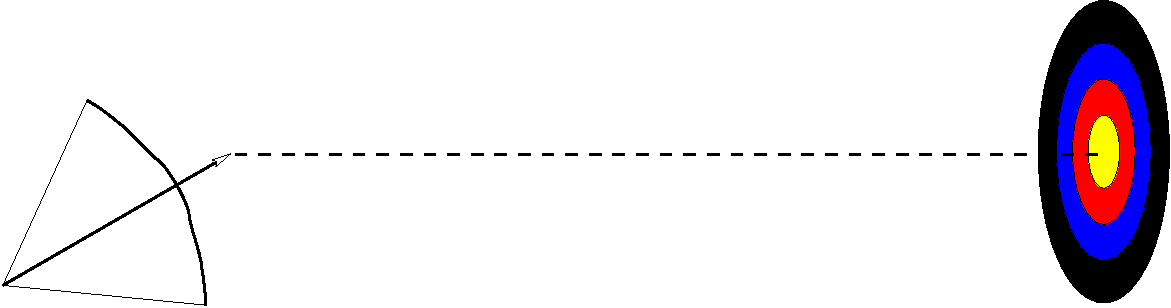
\includegraphics[width=0.6\textwidth]{./Figures/target.pdf}
\end{center}
\end{application}

For our modelling, we assume that the tip of the arrow is exactly level with the bullseye when it is loosed, cf. the sketch above. The target is 30 metres away. Then the height of the arrow when it hits the target is
\[h(\alpha,v) = -\frac{4414.5}{\cos^2(\alpha) \, v^2} + 30 \, \tan\alpha \:. \]
Here, $h=0$ corresponds to hitting the bullseye. There are different possibilities for defining a measurement of ``instability'', and Alice decides to use 
\[ f(\alpha,v) = h_{\alpha}^2 + 3 h_v^2 \]
since she finds controlling the velocity more difficult than controlling the angle. The symbols $h_\alpha$ and $h_v$ are the partial derivatives of $h$ and will be defined in the next section. After familiarising yourself with that concept, convince yourself that $f$ as defined above can be considered a measure of instability of\footnote{What does it mean for a derivative to be large at a point? It means that a small change of the variable will have a large effect!} $h$. In this chapter, we will learn how to minimise functions like $f$ (instability) under constraints like $h=0$ (hitting the bullseye). The optimal angle and velocity for Alice's target practice are
\[\alpha^* = 44.70^{\circ} \:,\quad v^* = 17.16 \tfrac{m}{s} \:. \]

The fact that those numbers do not agree with how archers usually shoot is due to our assumptions and our modelling: wind was neglected, it was assumed that initially the tip of the arrow and the bullseye are exactly level, that the archer can do the maths and control the angle and velocity exactly, etc. -- in the absence of these assumptions, a very strong shot almost directly aimed at the bullseye is the most straightforward option. However, understanding the above methods is a first step towards more complex real-life applications such as the design of mechanical machines.

\section{Multivariate Functions and Partial Derivatives}

\begin{definition}[Functions of Several Variables]
A \emph{function of two variables} is a rule $f$ that assigns to each pair $(x,y)$ in a set $D\subseteq\mathbb{R}^2$ a unique real number $f(x,y)$. The set $D$ is called the \emph{domain} of $f$ and also denoted $D(f)$. The \emph{range} of $f$ is the set of values it maps to,
\[
R(f) = \left\{ z \in \mathbb{R} \: | \: z = f(x,y)\text{~for some~}(x,y)\in D  \right\} \:.
\]
Similarly, a \emph{function of $n$ variables} is a rule $f$ that assigns a unique real number $f(x_1,x_2,\dots,x_n)$ to each $(x_1,x_2,\dots,x_n) \in D\subseteq\mathbb{R}^n$.
\end{definition}

\begin{remark}
\begin{enumerate}[(i)]
	\item Writing $z=f(x,y)$, we call $x$ and $y$ the independent variables, and $z$ the dependent variable. Functions of several variables are also called \emph{multivariate functions}.
	\item Unless specified otherwise, the domain is always the largest set of points $(x,y)$ at which the expression that defines $f$ can be evaluated.
	\item Functions of two variables can be visualised as surfaces/graphs in $\mathbb{R}^3$: The domain is a subset of the $xy$-plane and for $(x_0,y_0)$ in that domain, we mark a point of height $f(x_0,y_0)$ over/under $(x_0,y_0)$. That is, the point of the graph with $(x,y)$-coordinates $(x_0,y_0)$ will have $z$-coordinate $z_0=f(x_0,y_0)$.
	\item Restriction to lines in the domain is an important technique for working with multivariate functions, cf. part (iv) of the following set of examples.
\end{enumerate}
\end{remark}

\begin{example}
\label{expl:first_graphs}
\begin{enumerate}[(i)]
\item Draw the graph of $f(x,y) = x^2 + y^2$.\\
{\it Sol.:}
%\figbox{Graph of $f$ (paraboloid) with curves from parts (iv) and (v) (3D):}
\begin{center}
	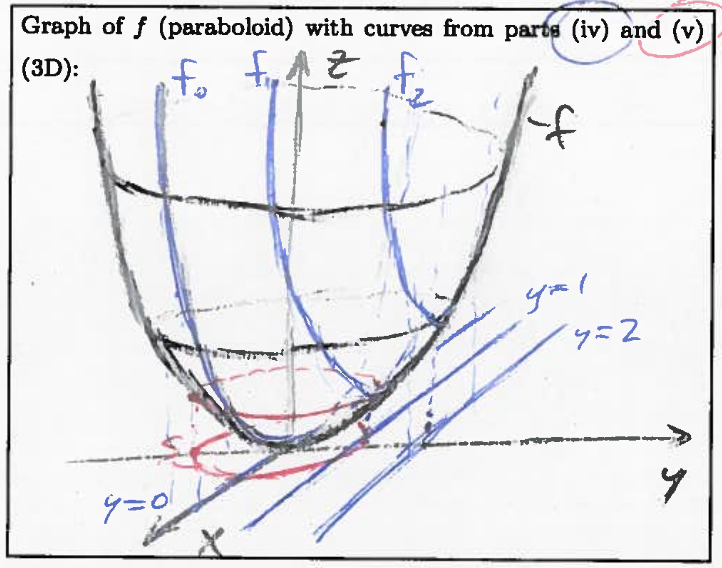
\includegraphics[width=0.6\textwidth]{./Figures/f301.png}
\end{center}
\item Find the domain and range of $g(x,y)= 1 + \sqrt{y-x^2}$.\\
{\it Sol.:}
The function $g$ is defined on the set
\[ D(g) = \left\{ (x,y) \in \mathbb{R}^2 \: | \: y \ge x^2 \right\} = \left\{ y \ge x^2 \right\} \:, \]
since we need $ y-x^2 \ge 0$ to be able to evaluate the square root. On this domain, the argument of the square root takes all non-negative real values $t\in[0,\infty)$, producing non-negative real numbers $\sqrt{t}\in[0,\infty)$. Therefore, the range is $R(g) = [1, \infty).$
\item Find the domain and range of $h(x_1,x_2,x_3)= \sin (x_1x_2+x_3)$.\\
{\it Sol.:}
The domain is $D = \mathbb{R}^3$ since $h$ can be evaluated at any $(x_1,x_2,x_3)$. The range of $h$ is $R = [-1,1]$.
\item Draw the graphs of the following one-variable functions
\begin{equation*}
\begin{split}
f_0(x) & = x^2 \:, \\
f_1(x) & = x^2 + 1 \:, \\
f_2(x) & = x^2 + 4 \:.
\end{split}
\end{equation*}
Where do these curves appear in the graph in (i)?\\
{\it Sol.:}
The functions $f_0,f_1,f_2$ are restrictions of $f(x,y)$ in (i) to the lines $y=0,y=1,y=2$. This can also be expressed as
\begin{equation*}
\begin{split}
f_0(x) & = f(x,0) = x^2 + 0^2 \:, \\
f_1(x) & = f(x,1) = x^2 + 1^2 \:, \\
f_2(x) & = f(x,2) = x^2 + 2^2 \:.
\end{split}
\end{equation*}
%\figbox{Graphs of $f_0,f_1,f_2$ (compare to graph (i); 2D):}
\begin{center}
	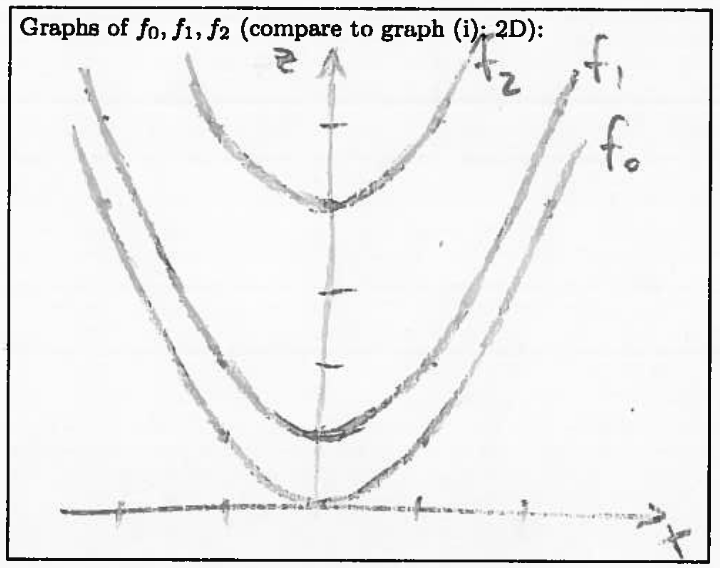
\includegraphics[width=0.6\textwidth]{./Figures/f302.png}
\end{center}
\item The domain of the function $f(x,y) = x^2 + y^2$ from (i) is $D(f)=\mathbb{R}^2$. Describe the subset $S$ of points in $D$ with $f(x,y)=1$.\\
{\it Sol.:} The equation
\[ x^2 + y^2 = 1 \]
defines a circle in the $xy$-plane:
%\figbox{Curve $S$ in $xy$-plane (compare to graph (i); 2D):}
\begin{center}
	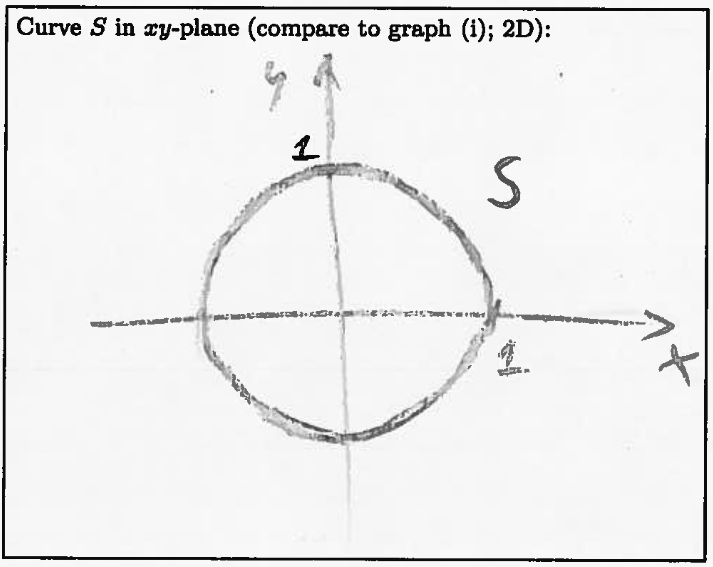
\includegraphics[width=0.6\textwidth]{./Figures/f303.png}
\end{center}
\end{enumerate}
\end{example}

\begin{definition}[Partial Derivatives]
For a function $f$ of two variables, the \emph{partial derivatives} with respect to $x$, respectively $y$, are the functions 	
\begin{equation*}
\begin{split}
\df{f}{x}(x,y) & = \lim_{h\to 0} \frac{f(x+h,y)-f(x,y)}{h} \:, \\
\df{f}{y}(x,y) & = \lim_{h\to 0} \frac{f(x,y+h)-f(x,y)}{h} \:.
\end{split}
\end{equation*}
We also write $f_x$ for $\df{f}{x}$ and $f_y$ for $\df{f}{y}$. Similarly for functions of more than two variables:
\begin{equation*}
\df{f}{x_j}(x_1,x_2,\dots,x_n) = \lim_{h\to 0}
\frac{f(x_1,x_2,\dots,x_{j-1},x_j+h,x_{j+1},\dots,x_n)-f(x_1,x_2,\dots,x_n)}{h} \:. \\
\end{equation*}
\end{definition}

\begin{example}
Find $f_x$ for the function $f(x,y) = 5x^2y^7$.\\
{\it Sol.:}
\begin{equation*}
\begin{split}
\df{f}{x}(x,y) & = \lim_{h\to 0}  \frac{f(x+h,y)-f(x,y)}{h} \\
& = \lim_{h\to 0}  \frac{5(x+h)^2y^7-5x^2y^7}{h} \\
& = 5y^7 \lim_{h\to 0} \frac{(x+h)^2 - x^2}{h} \\
& = 5y^7 \lim_{h\to 0} \frac{x^2+2hx+h^2 - x^2}{h} \\
& = 5y^7 \lim_{h\to 0} (2x+h) = 5(2x)y^7 = 10xy^7 \:.
\end{split}
\end{equation*}
The factor $2x$ in the last line is just the ordinary single-variable derivative of the factor $x^2$ of $f$. That is, the operator $\rfrac{\partial}{\partial x}$ differentiates the $x$-dependent part of $f$ in the usual way and treats terms that do not depend on $x$ as constants:
\begin{equation*}
\df{f}{x}(x,y) = \df{}{x} \left( 5x^2y^7\right) = 5 \, \df{}{x} \left( x^2\right) y^7 = 5(2x)y^7 = 10xy^7 \:.
\end{equation*}
\end{example}

\begin{example}
\begin{enumerate}[(i)]
	\item For $f = x^3 + y^5 - 2$, find $f_x$ and $f_y$.\\
	{\it Sol.:}
	\begin{equation*}
	\begin{split}
	f_x & = \df{}{x} \left( x^3 + y^5 - 2 \right) = 3x^2+0+0 = 3x^2 \:, \\
	f_y & = \df{}{y} \left( x^3 + y^5 - 2 \right) = 0+5y^4+0 = 5y^4 \:. 
	\end{split}
	\end{equation*}
	\item For $f=x^3+x^2y^3 -2 y^2$, find $f_x$ and $f_y$.\\
	{\it Sol.:}
	\begin{equation*}
	\begin{split}
	f_x & = \df{}{x} \left( x^3 \right) + \df{}{x} \left( x^2 \right)y^3 - 0 = 3x^2 +2xy^3 \:, \\
	f_y & = 0 + x^2 \df{}{y} \left( y^3 \right) - 2 \df{}{y}\left( y^2 \right) = 3x^2y^2 -4y \:. \\
	\end{split}
	\end{equation*}
\end{enumerate}
\end{example}

\begin{remark}
\begin{enumerate}[(i)]	
\item For a geometric interpretation, we consider the graph of a function $f$ of two variables, i.e. $z = f(x,y)$. Then $\rfrac{\partial z}{\partial x}$ is the slope on the surface ``when moving in the $x$ direction''. That is, $x$ is varied, $y$ is held constant, and we take note of the change of function values. Similarly, $\rfrac{\partial z}{\partial y}$ is the slope in the $y$ direction. 

As an intuitive example, consider a hiker climbing a mountain of the shape $z = 4-(x^2+y^2)$. 
%\figbox{``Steep mountain'' with hiker's position and paths in $x$ and $y$ direction (3D):}
\begin{center}
	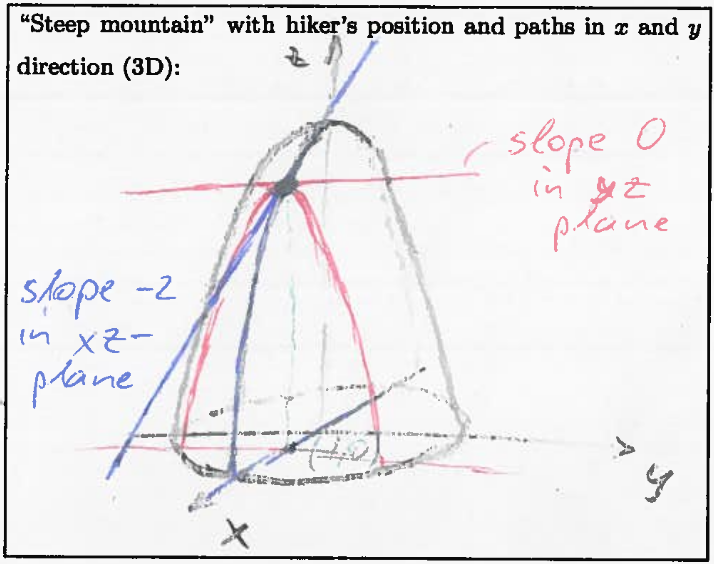
\includegraphics[width=0.6\textwidth]{./Figures/f304.png}
\end{center}
Suppose she checks her GPS and finds that her coordinates are $(x,y) = (1,0)$. The slopes at this point in both directions are
\begin{equation*}
\begin{split}
z_x(1,0) & = \df{}{x} \left( 4-(x^2+y^2) \right)_{|(x,y)=(1,0)} 
	= \left( -2x \right)_{|(x,y)=(1,0)} = -2 \:, \\
z_y(1,0) & = \df{}{y} \left( 4-(x^2+y^2) \right)_{|(x,y)=(1,0)} 
	= \left( -2y \right)_{|(x,y)=(1,0)} = 0 \:.
\end{split}
\end{equation*}
That is, there is no slope in the $y$ direction. The slope in the $x$ direction is negative, because the height decreases as $x$ increases (from where she stands, increasing $x$ would be moving away from the peak).
\item In order to be able to work with a larger set of functions -- not just sums of  products and powers of variables -- we extend the single-variable differentiation rules to the multivariate setting: The $x$-derivative of a product of functions is
\[ (fg)_x  = f_xg + fg_x \:, \]
that is, the product rule extends to partial derivatives without any changes. Similarly for $\rfrac{\partial}{\partial y}$. The quotient rule for a $y$-derivative is
\[ \left( \frac{f}{g} \right)_y = \frac{f_y g-f g_y}{g^2} \:. \]
\item In order to find partial derivatives of functions like
\[ f(x,y) = \sin(x+y^2) \:, \]
we also need to combine the chain rule for single-variable functions with partial derivatives. Note that the outer function, $h(t)=\sin(t)$, is a single-variable function. Let $c$ be a constant and review the following applications of the single-variable chain rule.
\begin{equation}
\label{eq:single-var_chain}
\begin{split}
\Df{}{t}\left(\sin(t+c)\right) & = \cos(t+c) \Df{}{t} (t+c) = \cos(t+c) \:,  \\
\Df{}{t}\left(\sin(c+t^2)\right) & = \cos(c+t^2) \Df{}{t} (c+t^2) = 2t\cos(c+t^2) \:.
\end{split}
\end{equation}
Now, the term $y^2$ looks like a constant to the operator $\rfrac{\partial}{\partial x}$. Similarly for $x$ and $\rfrac{\partial}{\partial y}$. We can thus apply the single-variable computations \eqref{eq:single-var_chain} to the two-variable function $f$ (in the first case, just replace $y^2$ with $c$):
\begin{equation*}
\begin{split}
f_x & = \df{}{x}\left(\sin(x+y^2)\right) = \cos(x+y^2) \df{}{x} (x+y^2) = \cos(x+y^2) \:,  \\
f_y & = \df{}{y}\left(\sin(x+y^2)\right) = \cos(x+y^2) \df{}{y} (x+y^2) = 2y\cos(x+y^2) \:.
\end{split}
\end{equation*}
This can be stated as
\[ \df{}{x} h(g(x,y)) = h'(g(x,y)) \cdot g_x(x,y) \:, \]
where $h$ is a single-variable function. Similarly for $\rfrac{\partial}{\partial y}$. Note that the $'$ is not ambiguous -- $h$ has only one variable, and $h'$ is the derivative with respect to (abbreviated: ``w.r.t'') that variable.
\end{enumerate}
\end{remark}

\begin{example}
\begin{enumerate}[(i)]
	\item The $y$-derivative of $f(x,y)=\e^{x^2+y^3}$ is found easily,
	\[ \df{}{y} \left( \e^{x^2+y^3} \right) 
	= \e^{x^2+y^3} \cdot \df{}{y}(x^2+y^3) = 3y^2 \, \e^{x^2+y^3} \:, \]
	and we can verify this result with the following alternative approach.
	\begin{equation*}
	\begin{split}
	\df{}{y} \left( \e^{x^2+y^3} \right) & = \df{}{y} \left( \e^{x^2}\e^{y^3} \right) = \e^{x^2} \df{}{y} \left( \e^{y^3} \right) \\
	& = \e^{x^2} \Df{}{y} \left( \e^{y^3} \right) = \e^{x^2} \e^{y^3} 3y^2 
	= 3y^2 \, \e^{x^2+y^3} \:. 
	\end{split}
	\end{equation*}
	Here, the ``$\partial$'' was changed to a ``$\d$'' to emphasise that in this approach, an ordinary derivative was taken, i.e., a derivative of a single-variable expression.
	\item 
	\[\begin{split}
	 \df{}{x}\left( \frac{\sin x \cos y }{x+y}\right) 
	& = \frac{\df{}{x}\Big(\sin x \cos y\Big) (x+y) - (\sin x \cos y)\df{}{x}\Big(x+y\Big)}{(x+y)^2} \\
	& = \frac{\cos y \left[ \cos x \cdot (x+y) - \sin x \right]}{(x+y)^2} 
	\end{split} \]
	\smallskip
\end{enumerate}
\end{example}

\begin{definition}[Higher-Order Partial Derivatives]
The \emph{second-order partial derivatives} with respect to $x$ and $y$ of a function $f$ of two variables are written
\begin{equation*}
\begin{split}
\ddf{f}{x} & = \df{}{x}\left( \df{f}{x}\right) , \\
\ddf{f}{y} & = \df{}{y}\left( \df{f}{y}\right) ,
\end{split}
\end{equation*}
and can also be denoted $f_{xx}$ and $f_{yy}$. We further have \emph{mixed} second-order derivatives:
\begin{equation*}
\begin{split}
\dff{f}{x}{y} & = \df{}{x}\left( \df{f}{y}\right) , \\
\dff{f}{y}{x} & = \df{}{y}\left( \df{f}{x}\right) .
\end{split}
\end{equation*}
Similarly for functions of more than two variables and for higher-order derivatives; e.g.,
\[ f_{xyyz} =\frac{\partial^4 f}{\partial x \partial y \partial y \partial z} 
		   = \df{}{x}\left(\df{}{y}\left(\df{}{y}\left(\df{f}{z}\right)\right)\right) \]
is a fourth-order derivative of a three-variable function $f=f(x,y,z)$.
\end{definition}

\begin{example}
\begin{enumerate}[(i)]
	\item
	For \[ f(x,y) = 2x^9y^5 \:, \] find all partial derivatives of order up to 2.\\
	{\it Sol.:}
	\begin{equation*}
	\begin{split}
	f & = 2x^9y^5 \:, \\
	f_x & = 2(9x^8)y^5=18x^8y^5 \:, \\
	f_y & = 2x^9(5y^4)=10x^9y^4 \:, \\
	f_{xx} & = \df{}{x} \left( 18x^8y^5 \right)=18(8x^7)y^5=144x^7y^5 \:, \\
	f_{yy} & = \df{}{y} \left( 10x^9y^4 \right)=10x^9(4y^3)=40x^9y^3 \:, \\
	f_{xy} & = \df{}{x} \left( 10x^9y^4 \right)=10(9x^8)y^4=90x^8y^4 \:, \\
	f_{yx} & = \df{}{y} \left( 18x^8y^5 \right)=18x^8(5y^4)=90x^8y^4 \:.
	\end{split}
	\end{equation*}
	\item
For \[f(x,y) = x^2 + 3xy - y^2 + 7x -4 y +2 \:, \] find \emph{all} partial derivatives.\\
{\it Sol.:}
\begin{equation*}
\begin{split}
f & = x^2+3xy-y^2+7x-4y+2 \:, \\
f_x & =  2x+3y+7 \:, \\
f_y & =  3x-2y-4 \:, \\
f_{xx} & = 2 \:, \\
f_{yy} & = -2 \:, \\
f_{xy} & = 3 \:, \\
f_{yx} & = 3 \:.
\end{split}
\end{equation*}
Since all the second-order derivatives are constant, all derivatives of higher order are zero,
\[ \frac{\partial^k f}{\partial \dots} = 0 \qquad \text{for~}k>2 \:. \]
	\item
	For \[ f(x,y) = x\, \cos(xy^2) \:, \] find all partial derivatives of order up to 2.\\
	{\it Sol.:}
	\begin{equation*}
	\begin{split}
	f & = x \cos(xy^2) \:, \\
	f_x & = \cos(xy^2) - xy^2 \sin(xy^2) \:, \\
	f_y & = -2x^2y \sin(xy^2) \:, \\
	f_{xx} & = -2y^2 \sin(xy^2) - xy^4 \cos(xy^2) \:, \\
	f_{yy} & = -2x^2 \sin(xy^2) - 4x^3y^2 \cos(xy^2) \:, \\
	f_{xy} & = -4xy \sin(xy^2) - 2x^2y^3 \cos(xy^2) = f_{yx} \:.
	\end{split}
	\end{equation*}
\end{enumerate}
\end{example}

\begin{remark}
In all of the previous examples, we had $f_{xy}=f_{yx}$. The following theorem states that this is not a coincidence -- it is always true as long as certain technical conditions are satisfied. Those conditions are met for the functions considered in this book, hence we can always work with the conclusion of the following theorem. However, be aware that there are functions that do not meet its requirements.
\end{remark}

\begin{theorem}[Schwarz's Theorem or Clairaut's Theorem]
\label{thm:schwarz}
Consider a function $f=f(x,y)$ and a point $(a,b)$ in its domain. If the functions $f_{xy}$ and
$f_{yx}$ are both continuous at $(a,b)$, then
\[f_{xy}(a,b)=f_{yx}(a,b) \:. \]
\end{theorem}

\begin{remark}
\texttt{Short remark on continuity for multivariate functions; or leave it -- depending whether 1D continuity is covered in chapter 1.}
\end{remark}

\begin{exercise}
\begin{enumerate}[(i)]
	\item Restrict the function $f(x,y)=xy$ to the lines $x=0$, $y=0$, $y=x$, $y=-x$. Hence draw the graph of\footnote{We have
	\[ f(x,x)=x^2\:, \quad f(x,-x) = -x^2 \:. \]
	That is, there is a parabola ``sitting'' on the line $y=x$ of the $xy$-plane and an upside-down parabola ``hanging'' under the line $y=-x$. The full graph looks like a saddle. You can use software to help visualising such functions; e.g., enter \texttt{plot x*y} in WolframAlpha. Note that, even though this is a curved surface, you can form it with straight lines (e.g., with mikado sticks) since the restriction of the graph to any $y=c$ is a line.} $f$.
	\item Find $f_x,f_y,f_{xx},f_{xy},f_{yy},f_{yx}$ for the functions\footnote{The $xy$ derivatives of the three functions are
	\[ 2x+12x^2y^3 \:, \quad \e^x \:, \quad -\sin x \, \tfrac{1}{y} \:, \]
	and we always have $f_{xy}=f_{yx}$. You can use software to check your results; e.g., \texttt{partial derivatives of \ldots} in WolframAlpha. Use such commands only to support your studies though -- do not rely on software!}
	\begin{enumerate}[(a)]
		\item $f(x,y) = x^2y+x^3y^4 + 7y \:;$
		\item $f(x,y) = y\,\e^x \:;$
		\item $f(x,y) = \cos x \ln y \:.$
	\end{enumerate}
	\item Find $f_x,f_y,f_{xx},f_{xy},f_{yy},f_{yx}$ for the functions\footnote{The $xy$ derivatives of the three functions are
		\[ \cos(xy+y^3) - y (x+3x^2) \sin(xy+y^3) \:, \quad
		-4xy - 2xy \ln xy \:, \quad 
		\tfrac{2y(1+x^2+y^2)^2-4xy(1+x^2+y^2)(2x)}{(1+x^2+y^2)^4} \:. \]
		(If you don't quite get those expressions, you may have forgotten to apply the product rule.)}
	\begin{enumerate}[(a)]
		\item $f(x,y) = \sin \left( xy + y^3 \right) \:;$
		\item $f(x,y) = \frac{x^2y^2}{2}-x^2y^2 \ln (xy) \:;$
		\item $f(x,y) = \frac{x}{1+x^2+y^2} \:.$
	\end{enumerate}
	\item Find the domain and the range of\footnote{You can check your domain with a WolframAlpha command of the form \texttt{plot ... >= 0}.} $f(x,y) =\sqrt{ 2 \sin x \sin y}$. 
		\item Let $D\subseteq\mathbb{R}^2$ be the open disk of radius $1$, $D = \{x^2 + y^2 < 1\}$. Define a function that is defined for $(x,y) \in D$, and another function that is defined on the \emph{complement} of $D$,
	\[D^c = \mathbb{R}^2 \setminus D = \{x^2+y^2 \geq 1 \} \]
	(read this as ``all points outside of $D$'')\footnote{For example: $\ln(1-x^2-y^2)$ and $\sqrt{x^2+x^2-1}$\:.}.
	\item Verify that
	\begin{enumerate}[(a)]
		\item $y(t,x) = \e^{-kn^2t}\sin(nx) \:$ satisfies $\: y_t=ky_{xx} \:;$
		\item $r(x,y,z) = \sqrt{x^2+y^2+z^2} \:$ satisfies
		$\: r_{xx}+r_{yy}+r_{zz} = \tfrac{2}{r} \:.$
	\end{enumerate}
	\item Find \emph{all} partial derivatives of\footnote{Use Theorem~\ref{thm:schwarz} to justify that your answer can be given in the form \[\frac{\partial^n}{\partial y^n} \frac{\partial^m f}{\partial x^m}=\dots \:, \] i.e. it can be assumed that $x$-derivatives are taken first.} $f(x,y) = \e^{2x+3y}$.
	\item Consider the function $f(x,y)=x^2(1-x^2)-y^2$. Find all points for which both the $x$- and the $y$-derivative is equal to zero. That is, find $(x_0,y_0)$ with\footnote{Setting both partial derivatives equal to zero gives you a (non-linear) system of two equations; solving it should lead to three points.} $f_x(x_0,y_0)=f_y(x_0,y_0)=0$.
\end{enumerate}
\end{exercise}


\section{Chain Rule and Implicit Differentiation}

\begin{remark}
\label{rem:composition}
\emph{Curves} in the $xy$-plane can be parametrised by writing $x$ and $y$ as single-variable functions of a third variable, usually $t$ (think of it as ``time''):
\[ (x,y) = (x(t),y(t)) \:. \]
We denote such curves $\gamma$,
\begin{equation*}
\begin{split}
\gamma \: : \: \mathbb{R} & \: \rightarrow \: \mathbb{R}^2 \\
t & \: \mapsto \: \gamma(t) = \left(x(t),y(t)\right) \:.
\end{split} 
\end{equation*}
A given function $f=f(x,y)$ can then be restricted to $\gamma$ -- this is carried out formally via a composition : define the single-variable function $F$ as
\[F(t) = \left(f\circ\gamma\right) (t) = f(\gamma(t)) = f(x(t),y(t)) \:. \]
Finding the derivative of $F$ is now an important and applicable task.

The distinction $f \leftrightarrow F$ is often not made to simplify notation. That is, the single-variable function of $t$ may be called $f$ as well. This reduces the number of function names needed to write out a computation, but it also carries potential for confusion since the symbol ``$f$'' would then used for two different mathematical objects. 
\end{remark}

\begin{example}
\label{expl:chainruleI}
\begin{enumerate}[(i)]
	\item Draw the curves
		\begin{equation*}
		\begin{split}
		\gamma_1 \: & : \quad (x(t),y(t)) = (t,t) \:, \\
		\gamma_2 \: & : \quad (x(t),y(t)) = (3\cos t,3\sin t) \:, \\
		\gamma_3 \: & : \quad (x(t),y(t)) = (t,1-t^2) \:, 
		\end{split}
		\end{equation*}
		and highlight the point corresponding to $t=0$ in each of them. \\
		{\it Sol.:} 
		%\figbox{The curves $\gamma_1,\gamma_2,\gamma_3$ (2D):}
		\begin{center}
			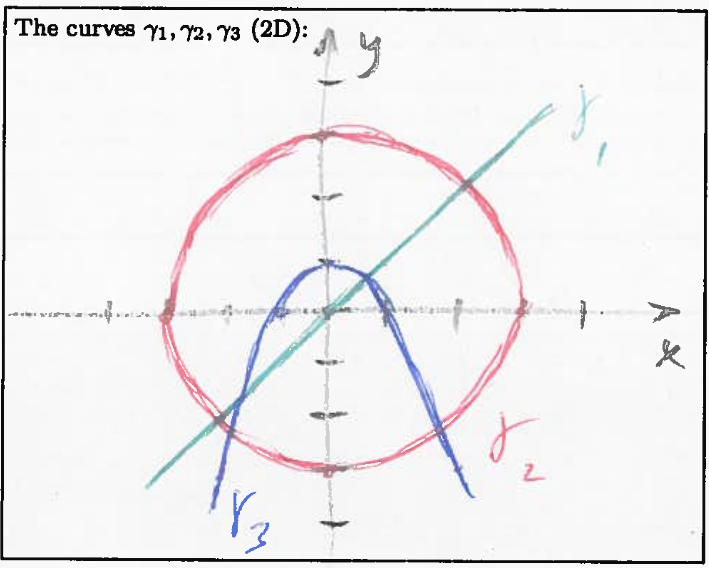
\includegraphics[width=0.6\textwidth]{./Figures/f305.png}
		\end{center}
	\item Consider the functions
		\begin{equation*}
		\begin{split}
		f_1 \: & : \quad f_1(x,y) = x-y \:, \\
		f_2 \: & : \quad f_2(x,y) = x^2+y^2 \:, \\
		f_3 \: & : \quad f_3(x,y) = \ln (3+x^2-y) \:, 
		\end{split}
		\end{equation*}
		and find the three single-variable functions $F_i=f_i\circ\gamma_i$.\\
		{\it Sol.:} 
		\begin{equation}
		\label{eq:chainruleI}
		\begin{split}
		F_1(t) & = \left(f_1\circ\gamma_1\right)(t) = f_1(t,t) = t-t = 0 \:, \\
		F_2(t) & = \left(f_2\circ\gamma_2\right)(t) = f_2(3\cos t, 3\sin t) 
		= (3\cos t)^2 +  (3\sin t)^2 = 9 \:, \\
		F_3(t) & = \ln \left( 3 + t^2 - (1-t^2) \right) = \ln \left( 2 + 2t^2\right) = \ln 2 + \ln\left(1+t^2\right).
		\end{split}
		\end{equation}
\end{enumerate}
\end{example}

\begin{theorem}[Chain Rule I]
\label{thm:CRI}
Let $f$ and $F$ be as in Remark~\ref{rem:composition}. Then
\[ \Df{F}{t} = \df{f}{x} \Df{x}{t} + \df{f}{y} \Df{y}{t} \:. \]
\end{theorem}

\begin{example}
\label{expl:chain_rule_i}
\begin{enumerate}[(i)]
	\item The derivatives of the functions $F_i$ in \ref{expl:chainruleI} are
\begin{equation*}
\begin{split}
\Df{F_1}{t} & = \df{f_1}{x} \Df{x}{t} + \df{f_1}{y} \Df{y}{t} 
= \df{(x-y)}{x} \Df{t}{t} + \df{(x-y)}{y} \Df{t}{t} = 1 \cdot 1 + (-1)\cdot 1 = 0 \:, \\
\Df{F_2}{t} & 
= 2x(t) \cdot (-3\sin t) + 2y(t) \cdot 3\cos t = -6 \cos t \sin t + 6 \sin t \cos t = 0 \:,  \\
\Df{F_3}{t} & = \frac{2x}{3+x^2-y} \cdot 1 + \frac{-1}{3+x^2-y} \cdot (-2t) 
= \frac{4t}{2+2t^2} = \frac{2t}{1+t^2} \:.
\end{split}
\end{equation*}
Alternatively, these derivatives could have been found by directly differentiating the functions $F_i=F_i(t)$ in \eqref{eq:chainruleI}. However, the chain rule allowed us to find the derivatives without using the explicit expressions of $t$ on the right-hand sides of \eqref{eq:chainruleI}, which is often very helpful.
	\item We now present an example in the simplified notation mentioned at the end of Remark~\ref{rem:composition}: For $f=x^2 y + 3x y^4$, $x=\sin 2 t$, $y= \cos t$,  find $\rfrac{\d f}{\d t}$ at $t=0$.
	{\it Sol.:}
\[ \Df{f}{t} = \df{f}{x} \Df{x}{t} + \df{f}{y}\Df{y}{t} 
= (2xy+ 3y^4)(2\cos 2t)+(x^2+12 xy^3)(-\sin t) \:. \]
The expressions containing the variable $t$ can be evaluated at $t=0$ directly. The other expressions we evaluate at the $x$ and $y$ values at $t=0$ : $x(0)=0$, $y(0)=1$. Therefore, the $t$-derivative of $f$ at $t=0$ is
\[ \Df{f}{t}(0) = 3\cdot 2 + 0 \cdot 0 = 6 \:. \]

To give this derivative a geometric interpretation, think of a hiker walking along the path $(x(t),y(t))$ in the ``mountain range'' that is given by the graph of $f$. Then our computations show that at time $t=0$, he will be climbing at a rate of six height units per time unit.
\end{enumerate}
\end{example}

\begin{remark}
\label{rem:transformations}
\emph{Changes of variables} in the $xy$-plane can be realised by writing $x$ and $y$ as functions of \emph{two} other variables,
\[ (x,y) = (x(s,t),y(s,t)) \:. \]
Given a function $f=f(x,y)$, one can then define a new function $F$ that has the same values as $f$, but is written out in term of $s$ and $t$ :
\[F(s,t) = f(x(s,t),y(s,t)) \:. \]
These changes of variables are quite useful -- for example, we will use them to solve differential equations in chapter \ref{ch:de} -- and it is important to be able to understand the relation of the partial derivatives of $f$ and $F$.

As in Remark~\ref{rem:composition}, the distinction $f \leftrightarrow F$ is sometimes not made, and the function of the new variables may be called $f$ as well. Again, this simplifies the notation but also carries potential for confusion. 
\end{remark}

\begin{theorem}[Chain Rule II]
\label{thm:CRII}
For $s,t,x,y,f,F$ as in Remark~\ref{rem:transformations}, we have
\begin{equation*}
\begin{split}
\df{F}{s} & = \df{f}{x}\df{x}{s} + \df{f}{y}\df{y}{s} \:, \\
\df{F}{t} & = \df{f}{x}\df{x}{t} + \df{f}{y}\df{y}{t} \:.
\end{split}
\end{equation*}
\end{theorem}

\begin{example}
\label{expl:chain_rule_ii}
\begin{enumerate}[(i)]
	\item Consider the function $f(x,y)=x-y$ and the change of variables 
	\[x(s,t)=s+t \:, \qquad y(s,t)=s-t \:. \]
	For $f$ in the new variables, i.e. $F(s,t)=f(x(s,t),y(s,t))$, we have partial derivatives 
	\begin{equation*}
	\begin{split}
	\df{F}{s} & = \df{f}{x}\df{x}{s} + \df{f}{y}\df{y}{s} = 1 \cdot 1 + (-1) \cdot 1 = 0 \:, \\
	\df{F}{t} & = \df{f}{x}\df{x}{t} + \df{f}{y}\df{y}{t} = 1 \cdot 1 + (-1) \cdot (-1) = 2 \:.
	\end{split}
	\end{equation*}
	As in the examples for derivatives along curves, the derivatives can be checked by explicitly writing out the function $F$ in terms of $s$ and $t$ :
	\[ F(s,t) = f(x,y) = x-y = (s+t)-(s-t) = 2t \:, \]
	which has the partial derivatives that were obtained above.
	\item Consider the paraboloid $f(x,y)=x^2+y^2$ and the change of variables
	\begin{equation}
	\label{eq:polar_coords}
	x(r,\theta)=r\cos\theta, \qquad y(r,\theta)=r\sin\theta \:.
	\end{equation}
	The partial derivatives of $F(r,\theta)=f(x,y)$ are
	\begin{equation*}
	\begin{split}
	\df{F}{r} & = \df{f}{x}\df{x}{r} + \df{f}{y}\df{y}{r} 
	= 2x \cdot \cos\theta + 2y \cdot \sin\theta 
	= 2r \left( \cos^2\theta + \sin^2\theta \right) = 2r \:, \\
	\df{F}{\theta} & = \df{f}{x}\df{x}{\theta} + \df{f}{y}\df{y}{\theta} 
	= 2r\cos\theta \cdot (-r\sin\theta) + 2r\sin\theta \cdot r\cos\theta = 0 \:.
	\end{split}
	\end{equation*}
	Again, we check these derivatives by explicitly writing out the function $F$ :
	\[ F(r,\theta) = f(x,y) = x^2+y^2 = r^2 \left( \cos^2\theta + \sin^2\theta \right) = r^2 \:, \]
	which confirms the partial derivatives that were found via chain rule II.
	
	The change of variables \eqref{eq:polar_coords} is the very important change to \emph{polar coordinates}. \texttt{Adjust this paragraph depending on whether polar coordinates are reviewed in the foundations chapter.}
	
	\item Let $g(s, t)=f(s^2-t^2, t^2-s^2)$, where $f$ is an arbitrary differentiable function. Show that $g$ satisfies
	\[ t\df{g}{s} + s \df{g}{t}=0 \:. \]
	{\it Sol.:}
	Let $ x=s^2-t^2, y=t^2-s^2$. Then,
	\begin{equation*}
	\begin{split}
	\df{g}{s} & = \df{f}{x} \df{x}{s} + \df{f}{y} \df{y}{s}=f_x \cdot 2s + f_y \cdot (-2s) \:, \\
	\df{g}{t} & = \df{f}{x} \df{x}{t} + \df{f}{y} \df{y}{t}=f_x \cdot (-2t) + f_y \cdot 2t \:.
	\end{split}
	\end{equation*}
	Therefore
	\[ t\df{g}{s} + s \df{g}{t}=0 \:. \]
	\item As in the examples \ref{expl:chain_rule_i} for chain rule I, we now present an example in simplified notation, where the function in the new variables is not given a new name. Consider the expression
	\begin{equation}
	\label{eq:first_pde_trafo}
	3\ddf{u}{x} +\frac12 \dff{u}{x}{y} -\frac12 \ddf{u}{y} 
	\end{equation}
	for the function $u=u(x,y)$, and rewrite it in terms of the new variables $\xi$ (``xi'') and $\eta$ (``eta'') defined as 
	\[ \xi=x+3y \:, \quad \eta=x-2y \:. \]
	{\it Sol.:} Chain rule II allows to rewrite the derivatives of $u$ with respect to $x$ and $y$ as derivatives w.r.t. $\xi$ and $\eta$ :
	\begin{equation*}
	\begin{split}
	\df{u}{x} &= \df{u}{\xi} \df{\xi}{x} + \df{u}{\eta} \df{\eta}{x}
	 = \df{u}{\xi} \cdot 1 + \df{u}{\eta} \cdot 1 = u_{\xi} + u_{\eta} \:, \\
 	\df{u}{y} &= \df{u}{\xi} \df{\xi}{y} + \df{u}{\eta} \df{\eta}{y}
	 = \df{u}{\xi} \cdot 3 + \df{u}{\eta} \cdot \left( -2 \right) 
	 = 3u_{\xi} - 2 u_{\eta} \:.
	 \end{split}
	\end{equation*}
	These formulas for the first-order derivatives of $u$ are only intermediate steps in our computation -- we need the second-order derivatives appearing in \eqref{eq:first_pde_trafo}: 
	\begin{equation*}
	\begin{split}
	\ddf{u}{x} & = \df{}{x}\left( \df{u}{x} \right)
		= \df{}{x} \left( u_{\xi} + u_{\eta} \right)
		= \df{u_{\xi}}{x} + \df{u_{\eta}}{x} \\
		& = \df{u_{\xi}}{\xi} \df{\xi}{x} + \df{u_{\xi}}{\eta} \df{\eta}{x}
		\: + \: \df{u_{\eta}}{\xi} \df{\xi}{x} + \df{u_{\eta}}{\eta} \df{\eta}{x} 
		 = u_{\xi\xi} + u_{\eta\xi} + u_{\xi\eta} + u_{\eta\eta} \:.
	\end{split}
	\end{equation*}
	Recalling Theorem~\ref{thm:schwarz}, we obtain
	\[ \ddf{u}{x} =  u_{\xi\xi} + 2 u_{\xi\eta} + u_{\eta\eta} \:. \]
	The second-order derivative w.r.t. $y$ is 
	\begin{equation*}
	\begin{split}
	\ddf{u}{y} &= \df{}{y}\left( 3u_{\xi} - 2 u_{\eta} \right)
	= 3\df{u_{\xi}}{y} -2 \df{u_{\eta}}{y} \\
	&= 3 \left( \df{u_{\xi}}{\xi} \df{\xi}{y} + \df{u_{\xi}}{\eta} \df{\eta}{y} \right)
-2 \left( \df{u_{\eta}}{\xi} \df{\xi}{y} + \df{u_{\eta}}{\eta} \df{\eta}{y} \right) \\
	&= 3\df{u_{\xi}}{\xi} \cdot 3 + 3\df{u_{\xi}}{\eta} \cdot \left( -2 \right)
	-2 \df{u_{\eta}}{\xi} \cdot 3
	-2 \df{u_{\eta}}{\eta} \cdot \left( -2 \right) \\
	&= 9 u_{\xi\xi} -12 u_{\xi\eta} + 4 u_{\eta\eta} \:.
	\end{split}
	\end{equation*}
	The mixed second-order derivative,
	\[ u_{xy} = 3 u_{\xi\xi} + u_{\xi\eta} - 2 u_{\eta\eta} \:, \]
	is obtained similarly. 
	This allows to write out \eqref{eq:first_pde_trafo} in terms of $\xi$ and $\eta$ :
	\begin{equation*}
	\begin{split}
	3\ddf{u}{x} & +\frac12 \dff{u}{x}{y} -\frac12 \ddf{u}{y} \\
	&= 3 \left[ u_{\xi\xi} + 2 u_{\xi\eta} + u_{\eta\eta} \right] 
	+\frac12 \left[ 3 u_{\xi\xi} + u_{\xi\eta} - 2 u_{\eta\eta} \right] 
	-\frac12 \left[ 9 u_{\xi\xi} - 12 u_{\xi\eta} + 4 u_{\eta\eta} \right] \\
	&= 0 \cdot u_{\xi\xi} + \left( 6 + \frac12 + 6 \right) \cdot u_{\xi\eta}
	+ 0 \cdot u_{\eta\eta} = \frac{25}{2} u_{\xi\eta} \:.
	\end{split}
	\end{equation*}
	Later, in Section \ref{sec:pdes}, we will use computations of this kind to solve a certain type of differential equation.
\end{enumerate}
\end{example}

\begin{definition}[Level Sets]
Given a function $f$ of $n$ variables and a constant $c$ in the range of $f$, the set of points in the domain of $f$ with
\[ f = c \]
is called a \emph{level set} of $f$. That is, a level set of $f$ is of the form
\[  \left\{ (x,y)\in\mathbb{R}^2 \: | \: f(x,y)=c \right\}\:.\]
\end{definition}

\begin{remark}
\begin{enumerate}[(i)]
	\item Level sets usually have one dimension less than the domain of the function. For example, the function $f(x,y) = x^2 + y^2$ is defined on the $xy$-plane, $\mathbb{R}^2$, which is two-dimensional. We have seen in Example~\ref{expl:first_graphs} that the condition
	\[ f(x,y) = x^2 + y^2 = 1 \]
	describes a curve, i.e. a one-dimensional object, namely the circle of radius $1$. In fact, $f(x,y)=x^2+y^2=c$ describes a one-dimensional object for any $c>0$. This may not work for all values of $c$ though: the only solution to $f=0$ is the point $(x,y)=(0,0)$, and points are considered zero-dimensional. The equation $f=c$, where $c<0$, has no solutions at all.
	
	Similarly, consider the function $f(x,y,z) = x^2 + y^2 + z^2$. It is defined in the three-dimensional space $\mathbb{R}^3$, and its level sets $f=c$ for $c>0$ are two-dimensional objects: spheres of radius $\sqrt{c}$ (the surfaces of the balls of radius $\sqrt{c}$ centred at the origin of the coordinate system).
	\item Considering $x$ and $y$ independent variables, we have
	\[ \df{y}{x} = 0 \]
	(the $x$-derivative of the function $g(x,y)=y$ is zero, since $g$ does not depend on $x$). 
	
	Now consider a level set $f(x,y)=c$. Under the constraint $f(x,y)=c$, the variables cannot both move freely any more. Such a level set is one-dimensional by the previous remark, i.e. a curve, and we can use $x$ as a parameter for it. That is, we let $x$ vary freely (independent variable) and then $y$ is determined (not independent any more) by the choice of $x$.
	
	For example, requiring $f_1 = 0$ in~\ref{expl:chainruleI} gives $y(x) = x$, and $f_3=\ln(2)$ gives $y(x)=1+x^2$.
\end{enumerate}
\end{remark}

\begin{theorem}[Implicit Differentiation]
\label{thm:impl_diff}
If the independent variable $y$ of the $xy$-plane $(x,y)\in\mathbb{R}^2$ is turned into a dependent variable $y=y(x)$ via a condition $f(x,y)=c$ (as in (ii) of the previous remark), then
\[ \Df{y}{x} = -\frac{f_x}{f_y} \:. \]
Similarly in $\mathbb{R}^3$: If the independent variable $z$ of $(x,y,z)\in\mathbb{R}^3$ is turned into a dependent variable $z=z(x,y)$ via a condition $f(x,y,z)=c$, then
\begin{equation*}
\begin{split}
\df{z}{x} = -\frac{f_x}{f_z} \:, \\
\df{z}{y} = -\frac{f_y}{f_z} \:. 
\end{split}
\end{equation*}
\end{theorem}

\begin{proof} Differentiating the condition $f(x,y(x))=c$ with respect to $x$ gives
\begin{equation}
\label{eq:pid1}
\Df{c}{x} = 0
\end{equation}
on the right-hand side. On the left-hand side, we use chain rule I to obtain
\begin{equation}
\label{eq:pid2}
\Df{f(x,y(x))}{x} = \df{f(x,y)}{x}\Df{x}{x} + \df{f(x,y)}{y}\Df{y}{x} \:.
\end{equation}
Note that here, $f$ appears as a function of one independent variable on the left, and as a two-variable function on the right. Since $\rfrac{\d x}{\d x} = 1$, combining~\eqref{eq:pid1} and~\eqref{eq:pid2} leads to the claimed formula for $\rfrac{\d y}{\d x}$.

Similarly, we differentiate the condition $f(x,y,z(x,y))=c$ with respect to $x$ and $y$,
\begin{equation*}
\begin{split}
\df{f(x,y,z(x,y))}{x} & = \df{f}{x}\df{x}{x} + \df{f}{y}\df{y}{x} +\df{f}{z}\df{z}{x} 
= f_x \cdot 1 + f_y \cdot 0 +f_z \cdot \df{z}{x} = 0 \:, \\
\df{f(x,y,z(x,y))}{y} & = \df{f}{x}\df{x}{y} + \df{f}{y}\df{y}{y} +\df{f}{z}\df{z}{y} 
= f_x \cdot 0 + f_y \cdot 1 +f_z \cdot \df{z}{y} = 0 \:,
\end{split}
\end{equation*}
to derive the other formulas stated in the theorem. The terms with $\rfrac{\partial y}{\partial x}$ and $\rfrac{\partial x}{\partial y}$ drop out by the previous remark. Here, $f$ appears as a two-variable function on the left and as a three-variable function in the other expressions.
\end{proof}
	
\begin{example}
\label{expl:impl_diff}
\begin{enumerate}[(i)]
	\item Find $\rfrac{\d y}{\d x}$ if $ x^3+y^3=6xy$.\\
	{\it Sol.:}
	\[ f(x,y)=x^3 + y^3 - 6xy = 0	
		\quad \Longrightarrow \quad \Df{y}{x} = -\frac{f_x}{f_y}= -\frac{3x^2-6y}{3y^2-6x} \:. \]
	\item Find $\tfrac{\partial z}{\partial x}$, $\tfrac{\partial z}{\partial y}$, $\tfrac{\partial^2 z}{\partial x \partial y}$, where $z=z(x,y)$ is defined by the equation
	\[ x+y-z=\e^z \:. \]
	{\it Method 1:} For $f(x,y,z)=x+y-z-\e^z$, we have
	\[f_x = \df{f}{x} = 1, \quad f_y= \df{f}{y} = 1, \quad
	f_z = \df{f}{z} = -1-\e^z \:. \]
	By Theorem~\ref{thm:impl_diff}, 
	\begin{equation*}
	\begin{split}
	\df{z}{x} & = - \frac{f_x}{f_z}= \frac{1}{1+\e^z} \:,\\
	\df{z}{y} & = - \frac{f_y}{f_z}= \frac{1}{1+\e^z} \:,
	\end{split}
	\end{equation*}
	and then, using the single-variable chain rule,
	\begin{equation*}
	\begin{split}
	\dff{z}{x}{y} & = \df{}{x} \left( \frac{1}{1+\e^z} \right) 
	= - \frac{1}{(1+\e^z)^2} \df{}{x} \left( \e^z \right) \\
	& = - \frac{\e^z}{(1+\e^z)^2} \df{}{x} \left( z \right)	= - \frac{\e^z}{(1+\e^z)^3} \:.
	\end{split}
	\end{equation*}
	{\it Method 2:} Differentiating both sides of $x+y-z=\e^z$ with respect to $x$ gives
	\[ 1 - \df{z}{x} = \e^z \df{z}{x} \:. \]
	Solving this for $z_x$, we find the same derivative as before.
	
	The two computations are very closely related -- Method~2 was presented to show that a more flexible approach can be used as well.
	\item For $z=u^v$, where $u=\sin x$ and $v=\cos x$, find $\rfrac{\d z}{\d x}$. \\
	{\it Sol.:} The chain rule for $z=z(x)$ reads
	\[
	\Df{z}{x} =\df{z}{u} \df{u}{x} + \df{z}{v} \df{v}{x}
	\:. \]
	The partials of $z = z (u,v)$ are
	\[
	\df{z}{u} = v u^{v-1}, \quad \df{z}{v}= u^v \ln u
	\:, \]
	and therefore
	\[
	\Df{z}{x} = v u^{v-1} \cos x - u^v \ln u \cdot \sin x
	=(\sin x)^{\cos x -1}  \cos^2 x -   \ln (\sin x) \cdot (\sin x)^{\cos x +1}
	\:. \]
	\item (Logarithmic Differentiation) Find $\rfrac{\partial z}{\partial x}$, $\rfrac{\partial z}{\partial y}$  for
	\begin{equation}
	\label{eq:symmetric_z}
	z=(x^2y+xy^2)^{\cos(xy)} \:.
	\end{equation} 
	{\it Sol.:}
	The idea for dealing with the function in the power on the right is to use the rule $\ln(a^p)=p\ln(a)$ for logarithms. If $a=b$, then $\ln(a)=\ln(b)$ -- applying this principle to~\eqref{eq:symmetric_z} gives
	\[
	\ln z = \ln\left( (x^2y+xy^2)^{\cos(xy)} \right) = \cos(xy) \ln(x^2y+xy^2)
	\:. \]
	Differentiating both sides with respect to $x$, we obtain
	\[
	\frac{1}{z} \df{z}{x} = -y \sin(xy) \ln(x^2y+xy^2)
	 + \cos(xy) \: \frac{2xy+y^2}{x^2y+xy^2}
	\]
	and
	\[
	\frac{\partial z}{\partial x} =  (x^2y+xy^2)^{\cos(xy)} \left[
	-y \sin (xy) \ln (x^2y+xy^2)+ \cos(xy) \: \frac{2x+y}{x^2+xy}
	\right]
	\:. \]
	The $y$-derivative of $z$ will be given as an exercise. It can be found analoguously, but it is much faster to point to the symmetry in~\eqref{eq:symmetric_z} and hence write down $\rfrac{\partial z}{\partial y}$ immediately.
\end{enumerate}
\end{example}

\begin{application}[Trajectories in phase space]
\texttt{Simple and quick example of a 2D phases space, e.g. for 1D motion; define energy on that phase space and find level curves.}
\end{application}

\begin{exercise}
	\begin{enumerate}[(i)]
		\item Find the rate of change of the functions
		\[ f(x,y) = x + x^2y - 5y^3\:, \quad g(x,y) = \sqrt{1+x^2+y^2} \]
		along the curve
		\[ \gamma(t) = (x(t),y(t)) = (t,t^2) \:. \]
		That is, find the $t$-derivatives of\footnote{
		\[ \begin{split}
		\Df{F}{t} & = \df{f}{x}\Df{x}{t} + \df{f}{y}\Df{y}{t}
		= (1+2xy) \cdot 1 + (x^2-15y^2) \cdot 2t \\
		& = 1 + 2 t t^2 + (t^2-15t^4)2t = 1 + 4 t^3 + 30 t^5 \\
		\Df{G}{t} & = \frac{t+4t^3}{\sqrt{1+t^2+t^4}}
		\end{split} \]
		} $F(t)=f(\gamma(t))$ and $G(t)=g(\gamma(t))$.
		\item Write the function $f(x,y) = x+y^2$ in polar coordinates, i.e. find an expression for $F=F(r,\theta)=f(x,y)$ in terms of $r$ and $\theta$. Then differentiate $F$ directly and compare to the $r$ and $\theta$ derivatives obtained via chain rule II (as in example~\ref{expl:chain_rule_ii} (ii)).
		\item Find $\rfrac{\partial z}{\partial x}$ and $\rfrac{\partial z}{\partial x}$
		for $z=z(x,y)$ defined by $z^3-3xyz=4 \:.$ 
		\item In Example~\ref{expl:impl_diff} (iv), the $x$-derivative of $z$ in~\eqref{eq:symmetric_z} was found by applying $\rfrac{\partial}{\partial x}$ to the logarithm of~\eqref{eq:symmetric_z}. Now find the derivative with respect to $y$ by repeating those steps. Comparing the two partial derivatives, try to interpret the reference to ``symmetry'' at the end of the example\footnote{In~\eqref{eq:symmetric_z}, the variable names $x$ and $y$ can be swapped, can't they? Having that in mind, what is the difference between the given $z_x$ and the $z_y$ you have found (they should be very similar -- if not, you have made a mistake)?}.
		\item Consider $u=u(x,y)$ and define the new variables $\xi=x-y$, $\eta=x+by$. Find $b$ so that the equation
		\[ \ddf{u}{x} +4\dff{u}{x}{y} +3\ddf{u}{y} = 0 \]
		transforms to\footnote{Carrying out the transformation as in Example~\ref{expl:chain_rule_ii}~(iv) leads to
		\[ 0 = 0 \cdot \ddf{u}{\xi} - 2(1+b) \cdot \dff{u}{\xi}{\eta} 
		+ (1+4b+3b^2) \cdot \ddf{u}{\eta} \:. \]
		The equation $u_{\xi\eta}=0$ we need to transform to has only a mixed derivatives. Hence $b$ needs to be chosen such that $1+4b+3b^2=0$. We choose $b=-\rfrac13$, since the other solution would also make the mixed derivative disappear. This gives $\rfrac{-4}{3}u_{u_{\xi\eta}}=0$; now multiply by $\rfrac{-3}{4}$.} $u_{\xi\eta}=0$.
		\item Consider $u=u(x,y)$ and the new variables $s,t$ defined by $x = \e^s \cos t$, $y = \e^2 \sin t$. Show that\footnote{This requires quite a bit of work. Start with
		\[ u_s = \df{}{s}(u) = \df{u}{x}\df{x}{s} + \df{u}{y}\df{y}{s} 
		= \e^s \left( u_x \cos t + u_y \sin t \right) \:. \]
	We need the product rule for the second $s$-derivative:
	\[ u_{ss} = \df{}{s}(u_s) = \df{}{s} (\e^s) \cdot \left( u_x \cos t + u_y \sin t \right)
	+ \e^s \left( \df{u_x}{s} \cos t + \df{u_y}{s} \sin t \right). \]
	Now find the $s$-derivatives of the functions $u_x,u_y$ by applying the chain rule -- as in the first step. Then simplify, repeat for $u_{tt}$, find the sum $u_{ss}+u_{tt}$.}
		\[ u_{xx} + u_{yy} = \e^{-2s}(u_{ss}+u_{tt}) \:. \]
		\item Find functions $f$ and corresponding constants $c$ such that the level sets $f=c$ are: a straight line of slope $+1$, a circle, a straight line of slope different from $\pm1$, a parabola, a hyperbola, an ellipse, two concentric circles, etc. Check your examples using software\footnote{For the hyperbola:
			\[ y = \frac{1}{x} \quad \longrightarrow \quad xy = 1 \quad \Longrightarrow
			\quad f(x,y)=xy \:,\:c=1 \:. \]
		Here is an example for the WolframAlpha syntax: \texttt{plot sin(x)*sin(y) = 0.1}~.}.
		\item Have the level set
		\[x^2(1-x^2) - y^2 = 0\]
		plotted and find the values of $x$ for which $\rfrac{\partial y}{\partial x} = 0$. What is the connection between those $x$-values and the plot of the level set\footnote{The level set is a curve of the shape of an infinity sign: $\infty\:$. The $y$-coordinate of its points can not be written as a function of $x$ since for most $x$, there are two corresponding $y$-values. Most individual segments of the curve can be written as $y(x)$ though (careful: this is not possible at $x=-1,0,1$), and then $y'(x_0)=0$ has the usual interpretation: a horizontal tangent line.}?
		\item Find the first-order partial derivatives of\footnote{You can \emph{check} (not ``find''!) your result with \texttt{differentiate z(x,y) = \ldots}}
		$z(x,y) = \left(\cos(2x)\right)^{\ln y}$.
		\item \texttt{Trajectory in phase space}
	\end{enumerate}
\end{exercise}


\section{Directional Derivatives and the Gradient Vector}

\begin{definition}[Gradient Vectors]
	The \emph{gradient vector} $\nabla f$ of a function $f(x,y)$ is the row vector containing its partial derivatives,
	\[ \nabla f = \begin{bmatrix} \df{f}{x} & \df{f}{y} \end{bmatrix} \:. \]
	Similarly for $f=f(x,y,z)$,
	\[ \nabla f = \begin{bmatrix} \df{f}{x} & \df{f}{y} & \df{f}{z} \end{bmatrix} \:. \]
\end{definition}

\begin{definition}[Directional Derivatives]
For a vector $v = \begin{bmatrix} a & b \end{bmatrix}^\top$ and a function $f$ of two variables, the \emph{directional derivative} of $f$ along $v$ is
\[ \mathrm{D}_v f = a \df{f}{x} + b \df{f}{y} 
= \nabla f \begin{bmatrix} a \\ b \end{bmatrix} \:, \]
and similarly for three-variable functions and directions $v = \begin{bmatrix} a & b & c \end{bmatrix}^\top$.
\end{definition}

\begin{example} Find the gradient of the function $f(x,y)=x\cos(y)-\sin(xy)$, and further its directional derivative along $v = \tfrac{1}{\sqrt{2}}\begin{bmatrix}
		1 & 1
	\end{bmatrix}^\top$ at the point $(x_0,y_0)=(\pi,0)$.\\
{\it Sol.:}
\begin{equation*}
\begin{split}
f(x,y) & = x\cos(y)-\sin(xy) \:, \\
\nabla f (x,y) & = 
\begin{bmatrix} \cos(y)-\cos(xy)y & -x\sin(y)-\cos(xy)x \end{bmatrix} \:, \\
\nabla f (x_0,y_0) & = 
\begin{bmatrix} \cos(0)-\cos(\pi 0)0 & -\pi\sin(0)-\cos(\pi 0) \pi \end{bmatrix}
= \begin{bmatrix} 1 & -\pi \end{bmatrix} \:, \\
\mathrm{D}_v f (0,\pi) & = \nabla f (x_0,y_0) \cdot v
= \frac{1}{\sqrt{2}}\begin{bmatrix} 1 & -\pi \end{bmatrix} 
\begin{bmatrix} 1 \\ 1 \end{bmatrix} = \frac{1-\pi}{\sqrt{2}} \:.
\end{split}
\end{equation*}
\end{example}

\begin{remark}
\label{rem:gradient_and_dd}
\begin{enumerate}[(i)]
	\item Consider a function $f=f(x,y)$ and a curve
	\[ \gamma(t) = \begin{bmatrix}
	x(t) \\ y(t)
	\end{bmatrix} \]
	in the $xy$-plane. (In the previous section, we had used the notation ``$(x(t),y(t))$'' for curves. Here, we simply switched from point notation $(x, y)$ for the points of $\gamma$ to vector notation $\begin{bmatrix} x & y \end{bmatrix}^\top$, cf. the application in Section~\ref{sec:rma}.) Define the function $F(t)=f(\gamma(t))=f(x(t),y(t))$. Then, comparing the definition of directional derivatives to chain rule I, we find
	\[ \Df{F}{t} = \df{f}{x}\Df{x}{t} + \df{f}{y}\Df{y}{t}
	 = \begin{bmatrix} f_x & f_y \end{bmatrix} \begin{bmatrix}	x' \\ y' \end{bmatrix}
	 = \mathrm{D}_{\gamma'}f , \]
	where prime dentotes the $t$-derivative and $\gamma'=\begin{bmatrix} x' & y' \end{bmatrix}^\top$.
	\item We introduce the following notation for the statement of the next theorem:
	\[ v \parallel w \]
	means that the vectors $v$ and $w$ are \emph{parallel}, i.e. one of them can be obtained from the other by scalar multiplication. The expression
	\[ v \perp w \]
	means that the two vectors are \emph{perpendicular} (or \emph{orthogonal}), i.e. the angle between them is $\rfrac\pi2$ ($90^\circ$ degrees). Reviewing section~\ref{sec:rma}, in particular remark~\ref{rem:vectors} and the definition before that, you will find:
	\[ v \perp w \quad \Longleftrightarrow \quad v \circ w = 0 \:. \]
	
	An important operation for vectors is to \emph{normalise} them: Given a vector $v$, we scalar-multiply it by the inverse of its length,
	\[ \bar{v} = \frac{1}{||v||} \cdot v = \frac{v}{||v||} \:, \]
	to obtain a vector $\bar{v}$ that (a) is parallel to $v$, i.e. points in the same direction, and (b) has unit length, $||\bar{v}||=1$. This is where the factor $\rfrac{1}{\sqrt{2}}$ of $v$ in the previous example comes from -- convince yourself that this vector has unit length! 
\end{enumerate}
\end{remark}

\begin{theorem}[Geometric Interpretation of Directional Derivatives]
\label{thm:geom_dd}
For vectors $v$ of length $||v||=1$, the absolute value of the directional derivative is maximal if $\nabla f ^\top \parallel v$, and zero if $\nabla f ^\top \perp v.$

In particular, level sets of a function are always perpendicular to the gradient of the function.
\end{theorem}
\begin{proof}
The directional derivative of $f$ along $v$ at the point $(x_0,y_0)$ is
\begin{equation*}
\begin{split}
\abs{\mathrm{D}_v f(x_0,y_0) }
& = \abs{ \nabla f (x_0,y_0) \cdot v} 
  = \abs{ \left( \nabla f (x_0,y_0) \right)^\top \circ v} \\
& \stackrel{\text{Remark}~\ref{rem:vectors}}{=}
 \abs{ \cos(\theta) \cdot || \left(\nabla f (x_0,y_0) \right)^\top || \cdot || v ||} 
  = \abs{ \cos(\theta) } \cdot || \left( \nabla f (x_0,y_0) \right)^\top || \:,
\end{split}
\end{equation*}
where $\theta$ is the angle between the vectors $v$ and $\left( \nabla f (x_0,y_0) \right)^\top$. The length of the latter is fixed, and only the cosine term can be changed by choosing a different vector $v$ of length 1. If the two vectors are parallel, then $\abs{\cos \theta} = 1$; if they are perpendicular, then $\abs{\cos \theta} = 0$; and for all other angles, $\abs{\cos \theta}$ will be between $0$ and $1$. This proves the first part of the statement.

For the second part, let the curve $\gamma(t)$ traverse a level set of $f$ and consider a fixed $t$-value $t_0$. Then $F(t)=f(\gamma(t))$ is constant, and therefore
\[ 0 = \Df{F}{t} (t_0) = \nabla f (x_0,y_0) \cdot \gamma'(t_0) = \left( \nabla f (x_0,y_0) \right)^\top \circ \gamma'(t_0) \:, \]
where $ \begin{bmatrix}
x'(t_0) & y'(t_0)
\end{bmatrix}^\top = \gamma'(t_0)$. This dot product being $0$ means that the two vectors are perpendicular. Since $\gamma'(t_0)$ is the tangent vector of the curve $\gamma(t)$ at $t_0$, we have completed the proof of the theorem.
\end{proof}

\begin{remark}
\begin{enumerate}[(i)]
	\item The same works in three dimensions: Then, a level set $f=c$ is a surface (two-dimensional), and the vector $\left(\nabla f\right)^\top$ will always be perpendicular to it.
	\item We now introduce a matrix of second-order derivatives that will be useful in the next section. For that, review Theorem~\ref{thm:schwarz}.
\end{enumerate}
\end{remark}

\begin{definition}[Hessian Matrix]
The \emph{Hessian matrix} or \emph{Hessian} of $f=f(x,y)$ is the matrix
\[ \mathrm{Hess} f = \begin{bmatrix}
f_{xx} & f_{xy} \\ f_{yx} & f_{yy}
\end{bmatrix} \:. \]
Similarly for functions of three or more variables. 
\end{definition}

\begin{example}
Find the gradient and the Hessian of $f(x,y,z) = xy^2 + z^3$.\\
{\it Sol.:}
\begin{equation*}
\begin{split}
\nabla f & = \begin{bmatrix}
y^2 & 2xy & 3z^2
\end{bmatrix},\\
\mathrm{Hess} f & = \begin{bmatrix}
0 & 2y & 0 \\
2y & 2x & 0 \\
0 & 0 & 6z
\end{bmatrix} \:.
\end{split}
\end{equation*}

\end{example}

\begin{exercise}
\begin{enumerate}[(i)]
	\item For $f(x,y) = \ln(x+y^2)$, find the gradient and the Hessian matrix at\footnote{
	\[\nabla f(3,1) = \frac{1}{4}\begin{bmatrix} 1 & 2 \end{bmatrix} \:, \quad
	 \mathrm{Hess}f(3,1)=\frac{1}{16}\begin{bmatrix} -1 & -2 \\ -2 & +4 \end{bmatrix} \]}
	$(x_0,y_0)=(3,1)$.
	\item Find the directional derivatives $D_vf(x_0,y_0)$ for\footnote{
	$D_vf(x_0,y_0)=\tfrac{63}{52};\:-\tfrac{7}{5};\:\tfrac{3-\pi}{2\sqrt{5}}.$}:
	\begin{enumerate}[(a)]
		\item $f(x,y)=y+\rfrac{x^2}{y}\:,\quad (x_0,y_0)=(1,2)\:,\quad
		v = \begin{bmatrix} \rfrac{12}{13} & \rfrac{5}{13}\end{bmatrix}^\top \:;$
		\item $f(x,y)=x^2-3xy+2y^2\:,\quad (x_0,y_0)=(1,1)\:,\quad
		v = \begin{bmatrix} \rfrac{3}{5} & -\rfrac{4}{5}\end{bmatrix}^\top \:;$
		\item $f(x,y)=x\arctan(\rfrac{y}{x})\:,\quad (x_0,y_0)=(1,-1)\:,\quad
		v = \begin{bmatrix} \rfrac{2}{\sqrt{5}} & \rfrac{1}{\sqrt{5}}\end{bmatrix}^\top \:.$
	\end{enumerate}
	\item Find the Hessian of $f(x,y)=\tfrac16\left((x-1)^3+(y+2)^3\right)$ at the point where\footnote{This quite a bit of work if you expand $f$, and a quick computation if you work with the given form. Answer: $I$.} $\nabla f=0$.
	\item For $f(x,y) = \left(\e^{3x}+\sin(4y) \right)^{5}$, find the unit vector $v$ (i.e., $||v||=1$) of steepest descent at\footnote{The steps for solving this are: Compare to theorem \ref{thm:geom_dd}, find the gradient of $f$ at the given point, normalise, choose one of the two possible directions.	Answer: $ v = \begin{bmatrix} -0.6 & 0.8 \end{bmatrix}^{\top}$.}
	$(x,y)=(0,\rfrac{\pi}{4})$.
	\item In remark \ref{rem:gradient_and_dd}, we have written out chain rule I as a matrix multiplication of a row vector and a column vector. Do the same for chain rule II: Find the matrix $M$ such that for the functions $f=f(x,y)$ and $F=F(s,t)$ in Theorem~\ref{thm:CRII} we have\footnote{The matrix $M$ contains the derivatives of the transformation $(s,t)\leadsto(x,y)$, cf. Theorem~\ref{thm:higher_dim_subst}.}
	\[  \nabla F = \nabla f \cdot M \:. \]
\end{enumerate}
\end{exercise}


\section{Taylor Approximations}

\begin{remark}
Recall single-variable Taylor approximations: For $F=F(t)$, we have the approximation
\[ F(t) \approx T_a^{(2)}F(t) = F(a) + F'(a)\cdot(t-a) + \frac{1}{2} F''(a)\cdot(t-a)^2 \]
close to the point $t=a$. In this section, we will derive the corresponding formula for functions of several variables.
\end{remark}

\begin{theorem}[Taylor Approximation]
Let $f(x,y)$ have continuous partial derivatives of order up to $2$, and let the point $(a,b)$ be in its domain. Then the \emph{first- and second-order Taylor approximations} of $f$ at $(a,b)$ are
\begin{equation}
\label{eq:TA}
\begin{split}
T_{(a,b)}^{(1)} f (x,y) = 
f(a,b) & + \nabla f (a,b) \begin{bmatrix} x-a \\ y-b \end{bmatrix} \:, \\
T_{(a,b)}^{(2)} f (x,y) = 
f(a,b) & + \nabla f (a,b) \begin{bmatrix} x-a \\ y-b \end{bmatrix} \\
 & + \frac{1}{2} \begin{bmatrix} x-a & y-b \end{bmatrix}
\mathrm{Hess} f (a,b) \begin{bmatrix} x-a \\ y-b \end{bmatrix} \:.
\end{split}
\end{equation}
Close to $(a,b)$, we have
\[ T_{(a,b)}^{(1)} f \approx f, \qquad T_{(a,b)}^{(2)} f \approx f \:, \]
where the second-order approximation is better in the sense that the error \[\abs{T_{(a,b)}^{(2)}f(x,y)-f(x,y)}\]
decays faster than $\abs{T_{(a,b)}^{(1)}f(x,y)-f(x,y)}$ as $(x,y)\to(a,b)$. Similarly for $f=f(x,y,z)$.
\end{theorem}

\begin{proof}
Let $(x,y)$ be close to the point $(a,b)$, so that both
\[ h = x-a \quad \text{and} \quad  k = y-b \]
are small. Define the curve
\[ \gamma(t) = (a+ht,b+kt) \:, \]
and let $F(t) = f(\gamma(t))$. Note that $\gamma(0)=(a,b)$ and $\gamma(1)=(x,y)$. We now find the second-order Taylor approximation of the single-variable function $F$ at $t=0$:
\begin{equation*}
\begin{split}
F(t) & \approx T_0^{(2)}F(t)
= F(0) + F'(0)\cdot t + \frac{1}{2} F''(0)\cdot t^2 \\
& = F(0) + t \cdot \Df{F}{t}(0) + \frac{1}{2}t^2 \cdot \Ddf{F}{t}(0) \\
& = f(a,b) + t \cdot \left[ \df{f}{x}\Df{x}{t} + \df{f}{y}\Df{y}{t} \right]_{t=0}
+ \frac{1}{2} t^2 \cdot \Df{}{t}\left[ \df{f}{x}\Df{x}{t} + \df{f}{y}\Df{y}{t} \right]_{t=0} \\
& = f(a,b) + t \cdot \nabla f (a,b) \begin{bmatrix} h \\ k \end{bmatrix}
+ \frac{1}{2} t^2 \cdot \Df{}{t}\left[ f_x \, h + f_y \, k \right]_{t=0} \:.
\end{split}
\end{equation*}
The remaining $t$-derivative is that of a composition with $\gamma$ (the evaluation at $t=0$ indicated as $[\dots]_{t=0}$ does not mean that $f_x$ and $f_y$ are evaluated at $t=0$ -- they are to be evaluated at $\gamma(0)=(a,b)$), and therefore, chain rule I needs to be applied one more time. Note that $h$ and $k$ do not depend on $t$.
\begin{equation*}
\begin{split}
\Df{}{t} \left[ f_x \, h + f_y \, k \right]_{t=0} 
& = h \cdot \left[ \df{f_x}{x} \Df{x}{t} + \df{f_x}{y} \Df{y}{t} \right] 
+ k \cdot \left[ \df{f_y}{x} \Df{x}{t} + \df{f_y}{y} \Df{y}{t} \right] \\
& = h^2 f_{xx} + hk f_{yx} + kh f_{xy} + k^2 f_{yy} \:,
\end{split}
\end{equation*}
where all the partials are evaluated at $(a,b)$. The last expression can be written as a matrix multiplication of the row vector containing $h$ and $k$, a matrix containing the second-order derivatives of $f$, and the column vector containing $h$ and $k$. This gives
\[
F(t) \approx f(a,b) + t \, \nabla f (a,b) \begin{bmatrix} h \\ k \end{bmatrix} 
+ \frac{t^2}{2} \begin{bmatrix} h & k \end{bmatrix}
\mathrm{Hess} f (a,b) \begin{bmatrix} h \\ k \end{bmatrix} \:.
\]
Evaluating this approximation at $t=1$, we obtain the stated second-order approximation of $f$,
\[
f(x,y) \approx f(a,b) + \nabla f (a,b) \begin{bmatrix} h \\ k \end{bmatrix} 
+ \frac{1}{2} \begin{bmatrix} h & k \end{bmatrix}
\mathrm{Hess} f (a,b) \begin{bmatrix} h \\ k \end{bmatrix} \:.
\]
Note that $t=1$ is not small, i.e. that it is not close to the point $t=0$ about which $F$ was developed, and that in general it may be too big for a good approximation. However, in the above situation, this can be controlled by requiring $h$ and $k$ to be small, that is, by letting $(x,y)$ be close to the point $(a,b)$ from which the approximation of $f$ is carried out.
\end{proof}

\begin{example}
\begin{enumerate}[(i)]
	\item Find the first- and second-order Taylor approximation of $f(x,y)=\e^x \ln(1+y)$ at $(a,b)=(0,0)$. \\
	{\it Sol.:} We begin by finding all the values, vectors, and matrices at $(a,b)$ that are needed for writing out the Taylor approximations \eqref{eq:TA}:
	\begin{equation*}
	\begin{split}
	f(x,y) & = \e^x \ln(1+y) \:, \\
	f(0,0) & = 1 \cdot 0 = 0 \:, \\
	\nabla f(x,y) & = \begin{bmatrix} \e^x \ln(1+y) & \frac{\e^x}{1+y} \end{bmatrix} \:, \\
	\nabla f(0,0) & = \begin{bmatrix} 0 & 1 \end{bmatrix} \:, \\
	\mathrm{Hess}f(x,y) & = \begin{bmatrix} \e^x \ln(1+y) & \frac{\e^x}{1+y} \:, \\
								 \frac{\e^x}{1+y} & -\e^x\frac{1}{(1+y)^2} \end{bmatrix} \:, \\
	\mathrm{Hess}f(0,0) & = \begin{bmatrix}	0 & 1 \\ 1 & -1	\end{bmatrix} \:.
	\end{split}
	\end{equation*}
	This gives
	\begin{equation*}
	T^{(1)}_{(0,0)}f(x,y) = f(0,0)+\nabla f(0,0) 
	\begin{bmatrix}	x-0 \\ y-0 \end{bmatrix}
	= 0 + \begin{bmatrix} 0 & 1 \end{bmatrix} \begin{bmatrix} x \\ y \end{bmatrix} = y
	\end{equation*}
	and
	\begin{equation*}
	\begin{split}
	T^{(2)}_{(0,0)}f(x,y) 
	& = 0 + \begin{bmatrix} 0 & 1 \end{bmatrix} \begin{bmatrix} x \\ y \end{bmatrix}
	+ \frac{1}{2} \begin{bmatrix} x & y \end{bmatrix}
	\begin{bmatrix}	0 & 1 \\ 1 & -1	\end{bmatrix}
	\begin{bmatrix} x \\ y \end{bmatrix} \\
	& = y + \frac{1}{2} \begin{bmatrix} x & y \end{bmatrix} 
	\begin{bmatrix} y \\ x - y \end{bmatrix} 
	= y + xy - \frac{y^2}{2} \:.
	\end{split}
	\end{equation*}
	\item Find the first- and second-order Taylor approximation of $f(x,y)= 2x^2 + y^2$ about the point $(a,b)=(1,1)$. \\
	{\it Sol.:}
	\begin{equation*}
	\begin{split}
	f(x,y) & = 2x^2 + y^2 \:, \\
	f(1,1) & = 3 \:, \\
	\nabla f(x,y) & = \begin{bmatrix} 4x & 2y \end{bmatrix} \:, \\
	\nabla f(1,1) & = \begin{bmatrix} 4 & 2 \end{bmatrix} \:, \\
	\mathrm{Hess}f(x,y) & = \begin{bmatrix} 4 & 0 \\ 0 & 2 \end{bmatrix} \:, \\
	\mathrm{Hess}f(1,1) & = \begin{bmatrix} 4 & 0 \\ 0 & 2 \end{bmatrix} \:,
	\end{split}
	\end{equation*}
	\begin{equation*}
	\begin{split} 
	T^{(2)}_{(1,1)}f(x,y) & = 3 + 
	\begin{bmatrix} 4 & 2 \end{bmatrix}
	\begin{bmatrix} x-1 \\ y-1 \end{bmatrix}
	+ \frac{1}{2} \begin{bmatrix} x-1 & y-1 \end{bmatrix}
	\begin{bmatrix} 4 & 0 \\ 0 & 2 \end{bmatrix}
	\begin{bmatrix} x-1 \\ y-1 \end{bmatrix} \\
	& = -3 + 4x + 2y + \begin{bmatrix} x-1 & y-1 \end{bmatrix}
	\begin{bmatrix} 2x-2 \\ y-1 \end{bmatrix} = 2x^2 + y^2 \:. 
	\end{split}
	\end{equation*}
	Note that we have obtained $T_{(a,b)}^{(2)}f=f$. This is because $f(x,y)$ is already a very simple function -- an expression of $x$ and $y$ containing terms of order at most $2$. The analogous situation in the corresponding single-variable theory is: The $m$-th-order Taylor approximation of a polynomial of order $d \leq m$ is the original polynomial itself. 
	
	It is important not to forget about one of the parts we were asked about -- the first-order approximation! It is contained in the above computation:
	\[ T^{(1)}_{(1,1)}f(x,y) = -3 +4x+2y \:. \]
	\item Find the second-order Taylor approximation of $f(x,y)= \sin(x)\sin(y)$ about the point $(a,b)=(\rfrac{\pi}{4},\rfrac{\pi}{4})$. \\
	{\it Sol.:}
    Note that $\sin(\rfrac{\pi}{4})=\cos(\rfrac{\pi}{4})=\rfrac{\sqrt{2}}{2}$. The required quantities at $(a,b)$ are
	\begin{equation*}
	\begin{split}
	f(x,y) & = \sin(x)\sin(y) \:, \\
	f(\rfrac{\pi}{4},\rfrac{\pi}{4}) & = \frac{1}{2} \:, \\
	\nabla f(x,y) & = \begin{bmatrix} \cos(x)\sin(y) & \sin(x)\cos(y) \end{bmatrix} \:, \\
	\nabla f(\rfrac{\pi}{4},\rfrac{\pi}{4}) 
	& = \begin{bmatrix} \frac12 & \frac12 \end{bmatrix} \:, \\
	\mathrm{Hess}f(x,y) & = \begin{bmatrix}
	-\sin(x)\sin(y) & \cos(x)\cos(y) \\ \cos(x)\cos(y) & -\sin(x)\sin(y) \end{bmatrix} \:, \\
	\mathrm{Hess}f(\rfrac{\pi}{4},\rfrac{\pi}{4}) 
	& = \frac{1}{2} \begin{bmatrix} -1 & 1 \\ 1 & -1 \end{bmatrix} \:.
	\end{split}
	\end{equation*}
	For simplicity, we write out the approximation in terms of $h=x-\rfrac{\pi}{4}$ and $k=y-\rfrac{\pi}{4}$:
	\begin{equation*}
	\begin{split}
	T^{(2)}_{(\rfrac{\pi}{4},\rfrac{\pi}{4})}f(x,y) 
	& = \frac{1}{2} + \frac{1}{2} \begin{bmatrix} 1 & 1 \end{bmatrix}
	\begin{bmatrix} h \\ k \end{bmatrix}
	+ \frac{1}{4} 	\begin{bmatrix} h & k \end{bmatrix}
	\begin{bmatrix} -1 & 1 \\ 1 & -1	\end{bmatrix}
	\begin{bmatrix} h \\ k \end{bmatrix} \\
	& = \frac{1}{2} \left[ 1 + h + k + hk - \frac{h^2}{2} - \frac{k^2}{2} \right] \:,
	\end{split}
	\end{equation*}
	which can then be translated back to an expression of $x$ and $y$ by replacing $h$ and $k$ with $x-\rfrac{\pi}{4}$ and $y-\rfrac{\pi}{4}$ respectively.
\end{enumerate}
\end{example}

\begin{remark}
\label{rem:taylor_appr}
\begin{enumerate}[(i)]
\item The second-order Taylor approximation of $f(x,y)$ at $(a,b)$ has the following properties (denote it by $T$ for simplicity: $T=T_{(a,b)}^{(2)}f$).
\begin{enumerate}[(a)]
	\item $T(a,b) = f(a,b)$ \hfill (same function value at $(a,b)$)
	\item $\nabla T(a,b) = \nabla f(a,b)$ \hfill (same first-order derivatives at $(a,b)$)
	\item $\mathrm{Hess}T(a,b) = \mathrm{Hess}f(a,b)$ \hfill (same second-order derivatives at $(a,b)$)
	\item $T$ is a second-order expression, i.e., a linear combination of $1,x,y,x^2,xy,y^2$.
\end{enumerate}
The last point should help you identify mistakes. For example, if you obtain terms like $x^2y$ or $y^5$ or $x \sin y$ in the approximation, you should review your computation -- forgetting to evaluate the gradient or the Hessian at the given point can lead to such expressions.
\item Similary, $T^{(1)}_{(a,b)}f$ is a first-order expression,
\[ T^{(1)}_{(a,b)}f = c_1 + c_2x +c_3y \:, \]
It further is a function of $x$ and $y$, of course, and we plot such functions in $\mathbb{R}^3$ by drawing the function values as the $z$-coordinate: 
\[ z = c_1 + c_2x +c_3y \:. \]
This is the equation of a plane in $\mathbb{R}^3$, namely the plane tangent to the graph of $f$ at the point $(x_0,y_0,z_0)=(a,b,f(a,b))$. This is similar to the corresponding 1D theory: The first-order Taylor approximation gives the equation of the tangent line.
%\figbox{Graphs of $f$ and $T^{(1)}_{(a,b)}f$ (3D):}
\begin{center}
	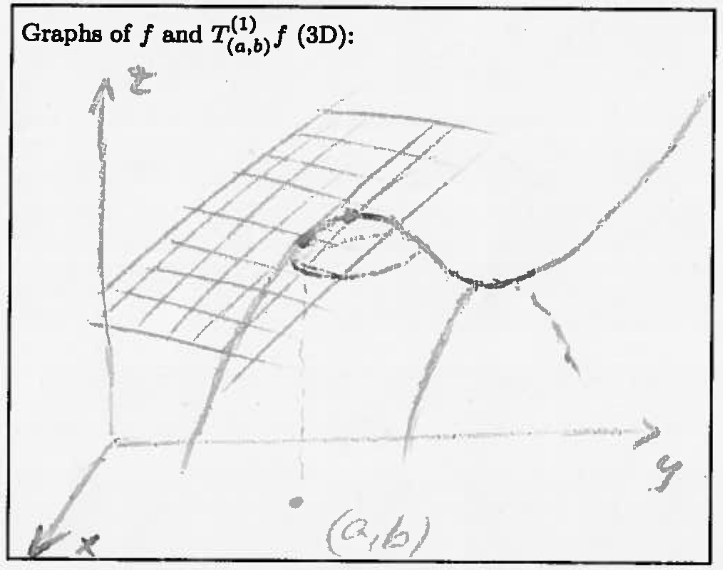
\includegraphics[width=0.6\textwidth]{./Figures/f306.png}
\end{center}
\end{enumerate}
\end{remark}

\begin{exercise}
\begin{enumerate}[(i)]
	\item Find the second-order Taylor approximation of $f(x,y)=x^2(1-y^3)$ at the point\footnote{
	\[ T_{(2,1)}^{(2)}f(x,y) = -12y^2-12xy+12x-36y-24 \]}
	$(a,b)=(2,1)$.
	\item Find the second-order Taylor approximation of $f(x,y,z)=xy^2+z^3$ at\footnote{You can verify your answer by checking the conditions in Remark~\ref{rem:taylor_appr}. To make sure that your second derivatives are correct, compare to the example at the end of the previous section.} $(a,b,c)=(1,1,1)$.
	\item Find the second-order Taylor approximation of $f(x,y)=\arctan(x+2y)$ at\footnote{
	\[ T_{(5,-2)}^{(2)}f(x,y) = -\frac{x^2}{4}-y^2-xy+x+2y+\frac{\pi-3}{4}\]}
	$(a,b)=(5,-2)$.
	\item Re-do example (ii) above, $f(x,y)=2x^2+y^2$, but now at a general point $(a,b)\in\mathbb{R}^2$. That is, use parameters $a$ and $b$ for the point at which the approximation is carried out, rather than specific numbers.
	\item Find the intersection of the $xy$-plane with the tangent plane of $f(x,y)=2x^2+y^2$ at\footnote{$y=x-\tfrac32.$} $(1,-2)$.
\end{enumerate}
\end{exercise}
	
	
\section{Local Extrema and Saddle Points}

\begin{definition}[Local Extrema and Critical Points]
For a function $f(x,y)$ and a point $(a,b)$ in its domain (similarly in three variables):
\begin{enumerate}[(i)]
	\item $(a,b)$ is a \emph{local maximum} of $f$ if 
	\[ f(x,y) \leq f(a,b) \]
	in some neighbourhood of $(a,b)$.
	\item $(a,b)$ is a \emph{local minimum} of $f$ if there exists an $\delta > 0$ such that
	\[ f(x,y) \geq f(a,b) \]
	for all $(x,y)$ with $\left|\left|\begin{bmatrix} x \\ y \end{bmatrix}
							   -\begin{bmatrix} a \\ b \end{bmatrix}\right|\right|<\delta$.
	\item $(a,b)$ is a \emph{critical point} of $f$ if 
	\[ \nabla f (a,b) = \begin{bmatrix} 0 & 0 \end{bmatrix} \:. \]
\end{enumerate}
\end{definition}

\begin{remark}
\begin{enumerate}[(i)]
	\item Neighbourhoods are small sets surrounding the point in question. For example, in one dimension: For $t_0 = 0.001$, there exists a small neighbourhood of $t_0$ that contains only positive numbers, e.g. the open interval $(t_0-0.0005,t_0+0.0005)$. For $t_0=0$, however, this is not possible: every neighbourhood -- no matter how small -- contains both positive and negative numbers. In the higher dimensional domains of multivariate functions, one can work with disks (in 2D) or balls (in 3D). This notion is very important in Mathematics and used informally in part (i) of the definition above. In part (ii), the same condition is written out more formally using a parameter $\delta$ and the corresponding disk of radius $\delta$ around the point $(a,b)$. It does not matter how small $\delta$ is, but $\delta>0$ is essential.
	\item A local extremum is either a local minimum or a local maximum. Local maxima are not surpassed in some small neighbourhood, while for local minima there exists a neighbourhood in which none of the other function values is smaller. There is no requirement for surrounding function values to be strictly smaller, respectively strictly larger -- that means, for example, that for a constant function $f(x,y)=c$, every point in its domain is both a local maximum and a local minimum.
	\item For the material in this section, it is useful to recall the corresponding single-variable theory. The following result should look familiar and its proof will be left as an exercise.
\end{enumerate}
\end{remark}

\begin{theorem}
\label{thm:crit_pts}
If $(a,b)$ is a local extremum of $f$, then $(a,b)$ is a critical point of~$f$.
\end{theorem}

\begin{example}
\label{expl:crit_points}
	\begin{enumerate}[(i)]
		\item Find the critical points of $f(x,y) = x^2y - y + 7$.\\
		{\it Sol.:}
		The gradient of $f$ is 
		\[  \nabla f (x,y) = \begin{bmatrix} 2xy & x^2-1 \end{bmatrix} \:. \]
		Setting its second component, i.e., the $y$-derivative of $f$, equal to zero, we obtain $x^2-1=0$, which has solutions $x=\pm1$. The second equation is $2xy=0$, which, since we know $x\not=0$, has the solution $y=0$. Therefore, the critical points are $(-1,0)$ and $(+1,0)$.
		\item Find the critical points of $f(x,y) = xy$.\\
		{\it Sol.:}
		Setting the gradient of $f$,
		\[  \nabla f (x,y) = \begin{bmatrix} y & x \end{bmatrix} \:, \]
		equal to zero gives the critical point $(a,b)=(0,0)$.
		
		Note, however, that this is not a local extremum: The function value at that point is $0$, and there are points with both positive and negative function values arbitrarily close to it. For example, consider the points $(x,y)=(\varepsilon,\varepsilon)$ and $(x,y)=(\varepsilon,-\varepsilon)$, where $\varepsilon$ is a small positive constant.
		\item Find the critical points of $f(x,y) = x^3 - 3x + 3xy^2$.\\
		{\it Sol.:}
		After computing the gradient of $f$, we find that $f_x=0$ for all points on the unit circle, and $f_y=0$ for all points that lie on one of the two axes. This gives the critical points $(+1,0)$, $(0,+1)$, $(-1,0)$, $(0,-1)$.
	\end{enumerate}
\end{example}

\begin{theorem}[Second-Derivative Test]
Let $(a,b)$ be a critical point of $f(x,y)$ and let 
\[ \Delta = \det \left( \mathrm{Hess} f (a,b) \right) 
= \left( f_{xx}f_{yy}-f_{xy}^2 \right)_{|(a,b)} \:. \]
Then $(a,b)$ can be classified as follows.
\begin{enumerate}[(i)]
	\item If $\Delta > 0$ and $f_{xx}(a,b)>0$, then $(a,b)$ is a local minimum.
	\item If $\Delta > 0$ and $f_{xx}(a,b)<0$, then $(a,b)$ is a local maximum.
	\item If $\Delta < 0$, then $(a,b)$ is not a local extremum.
	\item If $\Delta = 0$, then the test is inconclusive and $(a,b)$ could be any of the three possibilities above (local maximum, local minimum, or neither).
\end{enumerate}
\end{theorem}

\begin{example}
\label{expl:classifications}
\begin{enumerate}[(i)]
	\item Find and classify all critical points of $f(x,y) = x^2y - y + 7$.\\
	{\it Sol.:} In the previous example, we have found the critical points $P_1=(-1,0)$ and $P_2=(+1,0)$. The Hessian of $f$ is
	\[ \mathrm{Hess}f(x,y) =
	\begin{bmatrix}	2y & 2x \\ 2x & 0 \end{bmatrix} \:. \]
	At the first point, we have
	\[ \mathrm{Hess}f(P_1) =
	\begin{bmatrix}	0 & -2 \\ -2 & 0 \end{bmatrix} \:, \]
	which has determinant $\Delta = 0 \cdot 0 - (-2) \cdot (-2) = -4 < 0$. Hence, $P_1$ is neither a local maximum nor a local minimum. Points like $P_1$ are called \emph{saddle points}, cf. Remark~\ref{rem:schmiegquadriken}.
	At the second critical point, we have
	\[ \mathrm{Hess}f(P_2) =
	\begin{bmatrix}	0 & 2 \\ 2 & 0 \end{bmatrix} \:, \]
	which has determinant $\Delta = 0 \cdot 0 - 2 \cdot 2 = -4 < 0$. Hence, $P_2$ is a saddle point as well and therefore not a local extremum.
	\item Find and classify all critical points of $f(x,y) = x^3 - 3x + 3xy$.\\
	{\it Sol.:} Earlier we had found the critical points $P_1=(+1,0)$, $P_2=(0,+1)$, $P_3=(-1,0)$, and $P_4=(0,-1)$. The Hessian of $f$ is
	\[ \mathrm{Hess}f(x,y) =
	\begin{bmatrix}	6x & 6y \\ 6y & 6x \end{bmatrix} = 
	6\begin{bmatrix}	x & y \\ y & x \end{bmatrix} \:. \]
	This gives
	\[ \mathrm{Hess}f(P_1) = 6 I, \qquad \mathrm{Hess}f(P_3) = -6 I \:, \]
	which both have determinant $\Delta = +36 > 0$. Inspecting the signs of the entries in the upper left of those Hessians, we find that $P_1$ is a local minimum and that $P_3$ is a local maximum. At $P_2$ and $P_4$, we have
	\[ \mathrm{Hess}f(P_{2/4}) =
	\begin{bmatrix}	 0 & \pm6 \\ \pm6 & 0 \end{bmatrix} \:, \]
	which both have determinant $\Delta = -36 < 0$. Therefore, $P_2$ and $P_4$ are not local extrema.
	\item Find all critical points of 
	$f(x,y) = x - \ln x + 2 y^2 + xy$
	and classify them using the second derivative test.\\
	{\it Sol.:}
	\begin{equation*}
	\begin{split}
	f(x,y) &= x - \ln x + 2 y^2 + xy \:, \\
	\nabla f (x,y) & = \begin{bmatrix} 1 - \tfrac{1}{x} + y & 4y + x \end{bmatrix} \:,\\
	\mathrm{Hess}f(x,y) &= \begin{bmatrix} \rfrac{1}{x^2} & 1 \\ 1 & 4 \end{bmatrix} \:,\\
	P &= (2,-\tfrac{1}{2}) \:,\\
	\Delta &= 0 \:.
	\end{split}
	\end{equation*}
	Therefore, the second derivative test is inconclusive, and more work is required to classify the critical point $P=(2,-\tfrac{1}{2})$ of $f$.
\end{enumerate}
\end{example}

\begin{remark}
\label{rem:schmiegquadriken}
It is useful to understand the workings behind the second derivative test. We therefore sketch its derivation:

Since $(a,b)$ is a critical point of $f$, the second-order Taylor approximation	at that point is 
\[ T_{(a,b)}^{(2)} f (x,y) = f(a,b) + 0 
 + \frac{1}{2} \begin{bmatrix} x-a & y-b \end{bmatrix}
\mathrm{Hess} f (a,b) \begin{bmatrix} x-a \\ y-b \end{bmatrix} \:, \]
and it seems plausible that studying the approximation $T_{(a,b)}^{(2)}f$ should allow to classify $(a,b)$. Now, for the question whether $(a,b)$ is an extremum or not, overall additive constants such as the term $f(a,b)$ above do not matter. Also, we may shift our coordinate system so that $(a,b)\rightarrow(0,0)$. That is, we let $\wtd{x}=x-a$, $\wtd{y}=y-b$, as in the proof of the Taylor approximation, and we then write $\wtd{x}$ and $\wtd{y}$ as $x$ and $y$ again to simplify the notation. Thirdly, we denote the matrix $\tfrac12 \cdot \mathrm{Hess}f$ at the critical point by $M$. Note that $M$ is symmetric. With those steps, we have reduced classifying the critical point $(a,b)$ of the original function $f$ to classifying the critical point $(0,0)$ of the auxiliary function
\[ h(x,y) = \begin{bmatrix}	x & y \end{bmatrix} M 
\begin{bmatrix} x \\ y \end{bmatrix} \:. \]

More advanced theory of matrices implies that it suffices to restrict one's attention to the case when $M$ is a diagonal matrix. The basic idea for this argument is: if $M$ is not diagonal, then there is a change of variables so that $M$ written out in the new variables is diagonal. This change of variables is a rotation of the $xy$-plane, which does not affect the property of being a minimum, maximum, or neither. The function $h$ is now of the form
\[ h(x,y) = \begin{bmatrix}	x & y \end{bmatrix}  
\begin{bmatrix}	\lambda & 0 \\ 0 & \mu \end{bmatrix}
\begin{bmatrix} x \\ y \end{bmatrix} \:, \]
where $\lambda,\mu\in\mathbb{R}$. For example, consider the case $\lambda = 4$, $\mu = 1$. Then
\[ h(x,y) = 4 x^2 + y^2 = (2x)^2 + y^2 = \wtd{x}^2+y^2 \:, \]
where we rescaled the $x$ axis, $x \rightarrow \wtd{x} = 2x$. The expression on the right is a paraboloid, for which $(0,0)$ is a minimum. The rescaling causes a deformation -- imagine a paraboloid, then squeeze it so that its level sets are ellipses rather than circles -- but, again, this does not affect the property of having a minimum, maximum, or neither at the point $(0,0)$. We have therefore found that $h$ with $\lambda = 4$ and $\mu = 1$ has a local minimum at $(0,0)$. By this argument, we find that all the cases with $\lambda > 0$ and $\mu > 0$ are qualitatively the same and have a minimum. Let us choose the identity matrix as representing those cases,
\[ M_1 = I = \begin{bmatrix} 1 & 0 \\ 0 & 1 \end{bmatrix} \:, \]
for which $h(x,y)=x^2+y^2$ and the graph of $h$ is a paraboloid:
%\figbox{Example for case (i) ($h$ induced by $M_1$, paraboloid; 3D):}
\begin{center}
	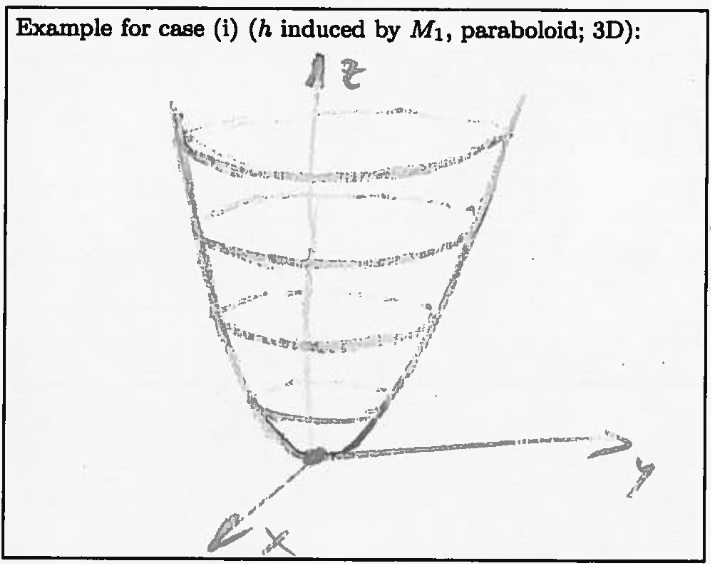
\includegraphics[width=0.6\textwidth]{./Figures/f307.png}
\end{center}
This is case (i) of the second derivative test, a local minimum. Note that the chosen representative $M_1=I$ for this class satisfies the assumptions of (i): $\det M_1 > 0$ and its upper left entry is positive.

Continuing this line of reasoning, one finds that the other cases to consider are:
\begin{equation*}
M_2 = \begin{bmatrix} -1 & 0 \\ 0 & -1 \end{bmatrix} \:,
M_3 = \begin{bmatrix} +1 & 0 \\ 0 & -1 \end{bmatrix} \:,
M_4 = \begin{bmatrix} +1 & 0 \\ 0 & 0 \end{bmatrix} \:, 
M_5 = \begin{bmatrix} -1 & 0 \\ 0 & 0 \end{bmatrix} \:, 
M_6 = \begin{bmatrix} 0 & 0 \\ 0 & 0 \end{bmatrix} \:.
\end{equation*}
The matrix $M_2$ generates the upside-down paraboloid $h(x,y)=-(x^2+y^2)$,
%\figbox{Example for case (ii) ($h$ induced by $M_2$, upside-down paraboloid; 3D):}
\begin{center}
	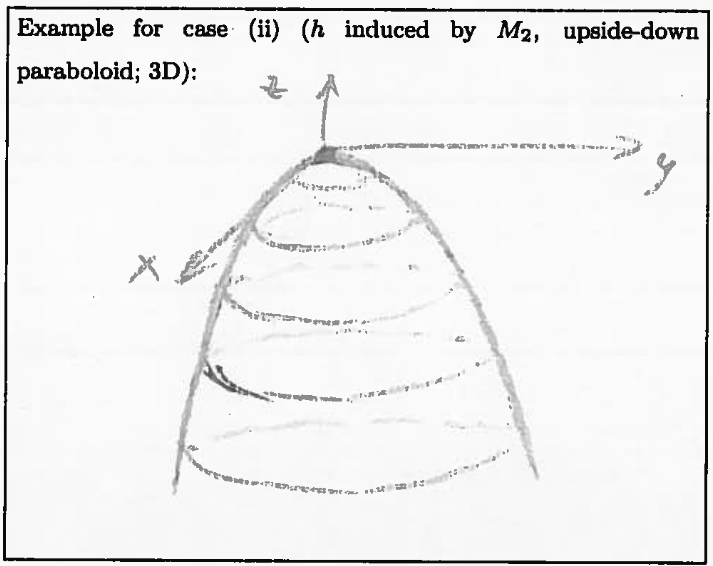
\includegraphics[width=0.6\textwidth]{./Figures/f308.png}
\end{center}
which has a maximum at $(0,0)$. Again, note that $M_2$ satisfies the assumptions of (ii) of the second derivative test. The matrix $M_3$ gives
\[ h(x,y) = x^2-y^2 \:, \]
which does not have an extremum at $(0,0)$: we have $h(0,0)=0$, but both positive and negative function values arbitrarily close (e.g. $h(\varepsilon,0)>0$ and $h(0,\varepsilon)<0$). This is case (iii) of the second derivative test, and both the graph of $h(x,y) = x^2-y^2$,
%\figbox{Example for case (iii), ($h$ induced by $M_3$, saddle; 3D):}
\begin{center}
	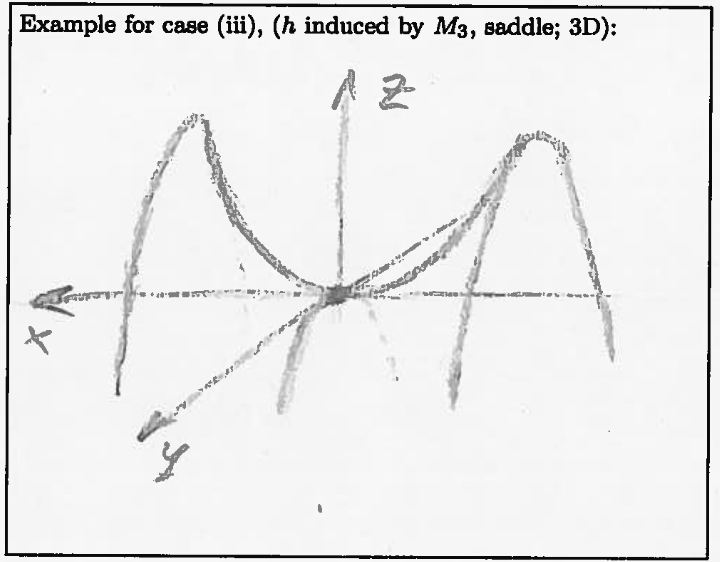
\includegraphics[width=0.6\textwidth]{./Figures/f309.png}
\end{center}
and the form of $M_3$ agree with the statements in (iii).

Finally, we argue that the cases represented by $M_4,M_5,M_6$ do not allow us to draw a conclusion, i.e. they correspond to case (iv) of the second derivative test. They all do satisfy the assumption $\det M = 0$. The choice $M_5$ gives $h(x,y)=-x^2$, which has the following graph.
%\figbox{Example for case (iv) ($h$ induced by $M_5$; 3D):}
\begin{center}
	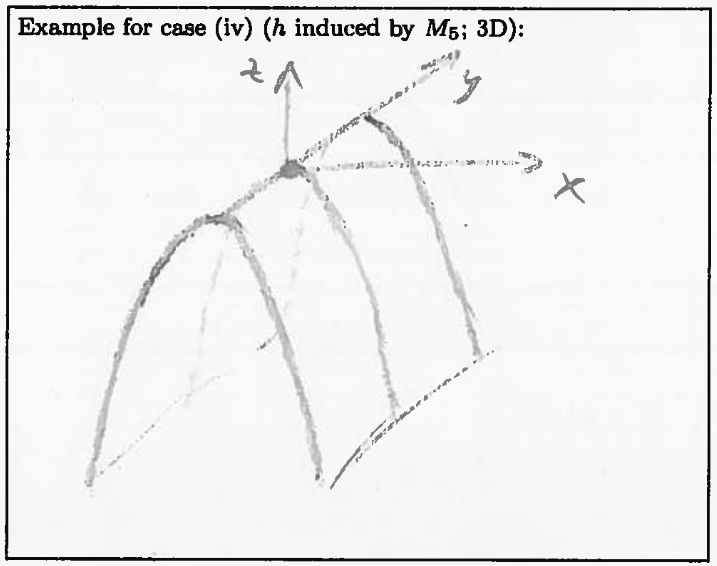
\includegraphics[width=0.6\textwidth]{./Figures/f310.png}
\end{center}
The matrix $M_4$ produces the same graph, but upside-down, and the graph obtained by choosing $M_6$ is the plane $h(x,y)=0$. In each of these cases, there is at least one straight line passing through the critical point $(0,0)$ in question. On this line, small contributions of the original function $f$, that are not captured by the second-order Taylor approximation, could tip the balance to different conclusions. Some guidance for understanding this will be provided in the exercises below.

The purpose of this remark was to explain the workings behind the second derivative test, to outline its proof, and, perhaps most importantly, to help avoid confusion of the cases (i) and (ii): For example, suppose you are classifying a critical point, you have obtained a Hessian matrix with positive determinant and positive entry in the upper left corner, but you have forgotten whether this implies a minimum or a maximum. Then think of the representative $M = I$ of this situation -- this gives the function $h(x,y) = x^2 + y^2$, which is the well-known paraboloid, which has a \emph{minimum} at $(0,0)$.
\end{remark}

\begin{application}[Mean squared error for linear regression]
\texttt{Define mean squared error for the linear regression application from the previous chapter; apply theory from the current chapter to basic matrix functions and hence show that linear regression minimises the MSE.}
\end{application}

\begin{exercise}
	\begin{enumerate}[(i)]
		\item Fill in the gaps for examples \ref{expl:crit_points} (iii) and \ref{expl:classifications} (iii), which were only sketched.
		\item Find an classify all critical points of\footnote{Only one critical point: a saddle point at $(-2,4)$.}
		$f(x,y) = x^2+xy+2y-1$. 
		\item Find and classify all critical points of\footnote{The critical points are
		\[ (0,0)\:,\quad(2,0)\:,\quad(1,1)\:,\quad(1,-1), \]
		and they are a maximum, minimum, saddle point, saddle point, respectively.}
		$f(x,y) = x^3+3xy^2-3x^2-3y^2-2$.
		\item Convince yourself that Theorem~\ref{thm:crit_pts} is true\footnote{You could contrapose that statement and/or look at Theorem~\ref{thm:geom_dd} for inspiration.}.
		\item Give examples of a local minimum, a local maximum, and a critical point that is neither, that cannot be classified with the second derivative test\footnote{$f(x,y)=x^4+y^4$ covers one of those cases.}.
	 	\item Use graphing software to explore different functions of the form
	 	\[ h(x,y) = \begin{bmatrix} x & y \end{bmatrix}
	 	M \begin{bmatrix} x \\ y \end{bmatrix} \:, \]
	 	where $M$ is a symmetric $2 \times 2$ matrix (i.e., $a_{12}=a_{21}$), and compare the different shapes you find to Remark~\ref{rem:schmiegquadriken}.
	 	\item For \ref{expl:classifications} (iii), use graphing software to find out what the point $P$ is\footnote{Classifying $P$ is quite difficult. Zooming in by appending \texttt{~for x from 1.99 to 2.01 and y from -0.51 to -0.49~} to the WolframAlpha plot command provides some insight.}.
	\end{enumerate}
\end{exercise}


\section{Extrema under Constraints: Lagrange Multipliers}

\begin{example}
\label{expl:naive_opt}
Find the maximum of the function $z=f(x,y)=2x+y$ on the circle $S = \{ (x,y) \in \mathbb{R}^2 \: | \: x^2+y^2=1 \}$, as well as the value that $f$ takes at that point.\\
{\it Sol.:} First note that the graph of $f$ is a plane, and therefore $f$ does not have any extrema at all on its full domain $\mathbb{R}^2$. However, a maximum does exist when restricting to the circle:
%\figbox{Maximum of $f$ on $S$ (3D):}
\begin{center}
	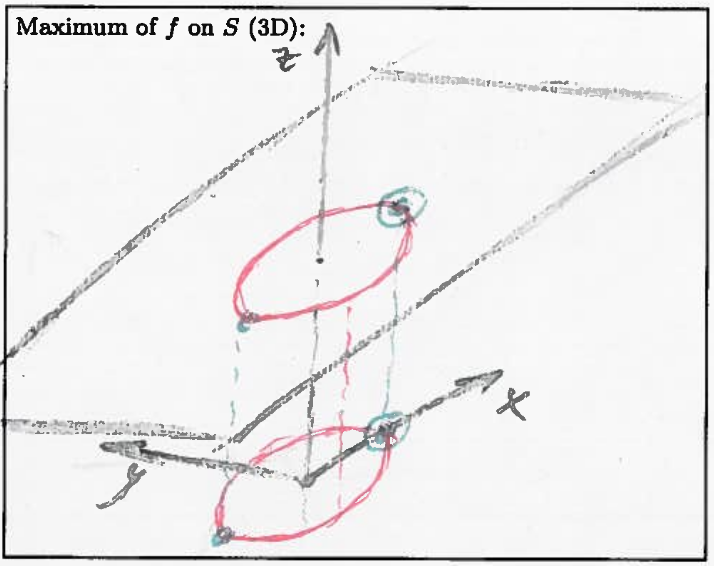
\includegraphics[width=0.6\textwidth]{./Figures/f311.png}
\end{center}
To find this point, we parametrise the circle as
\[ (x(t),y(t)) = (\cos(t),\sin(t)) \:, \]
and then define the function $F(t)=f(x(t),y(t))$. This gives
\begin{equation*}
\begin{split}
F(t) &= 2\cos(t)+\sin(t) \:, \\
F'(t) &= -2\sin(t)+\cos(t) \:.
\end{split}
\end{equation*}
Setting $F'(t)$ equal to zero, we obtain
\[ \tan(t_0) = \frac12 \:, \]
which has solutions $t_0 \approx 0.464 + k\pi$. Taking $k=0$ and $k=1$ leads to the points
\begin{equation*}
\begin{split}
(x_1,y_1)&\approx(\cos(0.464),\sin(0.464))\approx(0.894,0.448) \:, \\
(x_2,y_2)&\approx(\cos(3.606),\sin(3.606))\approx(-0.894,-0.448) \:,
\end{split}
\end{equation*}
and all other $k$ will yield one of those two points again. Evaluating, we see that $f$ has a larger value at $(x_1,y_1)$, and hence we obtain the answer: $f$ takes the maximum value $2.236$ on the circle $S$ at the point $(x,y)=(0.894,0.448)$.
\end{example}

\begin{remark}
Now suppose the set $S$ is given as a level set of a function $g$, and is less regular and can not be parametrised easily. The following figure shows such a set $S$ in the domain of $f$, and further a level set $f(x,y)=c$, where the constant $c=c_1$ is chosen to be larger than any of the values $f$ takes on $S$.
%\figbox{The level sets $g=0$ and $f=c$ for large $c$ (2D):}
\begin{center}
	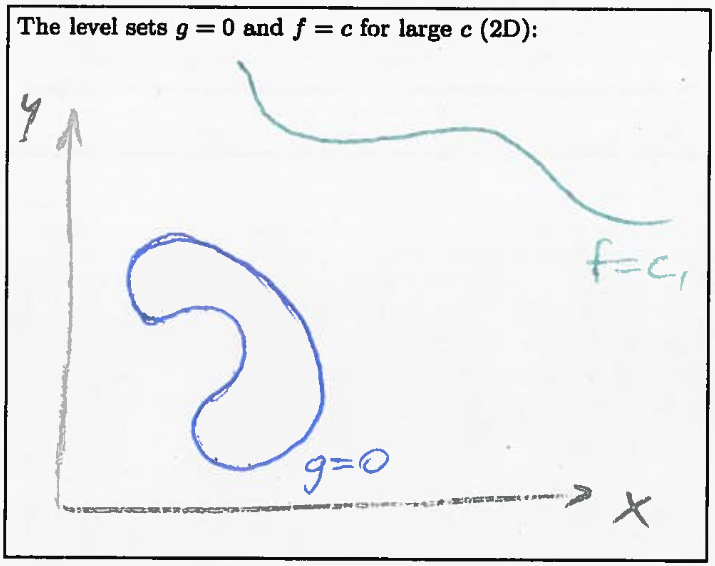
\includegraphics[width=0.6\textwidth]{./Figures/f312.png}
\end{center}
Now, choosing a slightly smaller constant $c_2$, the curve $f=c$ will move towards $g=0$. We continue this process until the first contact between the two curves is made, say for $c=c_3$. This contact point is a local maximum -- convince yourself of that\footnote{Can any of the other points in $S$ have larger function values?}!
%\figbox{The level sets $g=0$ and $f=c$ for smaller values of $c$ (2D):}
\begin{center}
	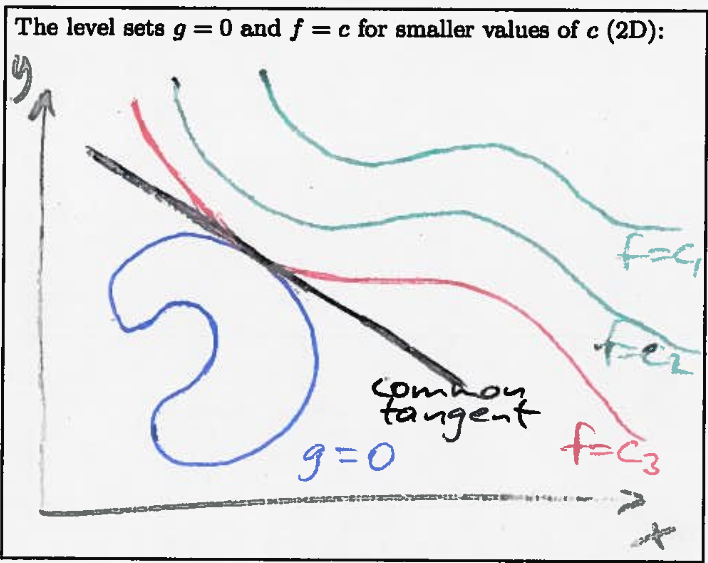
\includegraphics[width=0.6\textwidth]{./Figures/f313.png}
\end{center}
Note that the level curves $g=0$ and $f=c_3$ have a common tangent line -- convince yourself that this is always the case\footnote{Try to sketch a \emph{first-contact} scenario where the tangent lines at the contact point intersect (you will not succeed; be aware that level curves of smooth functions do not have ends -- they are either closed curves or they go out to infinity).}. Recall that gradient vectors are orthogonal to level sets and their tangent lines or planes. It must therefore be the case that the gradients of $f$ and $g$ are parallel:
\[ \nabla f = \lambda \nabla g, \qquad \text{for some~} \lambda \in \mathbb{R} \:. \]
\end{remark}

\begin{theorem}[Lagrange Multipliers]
To maximise or minimise a function $f(x,y)$ on a set 
$S = \{ (x,y) \in \mathbb{R}^2 \: | \: g(x,y) = 0 \} $,
define the function
\[ F(\lambda,x,y) = f(x,y) - \lambda g(x,y) \:, \]
and then solve
\[ \nabla F = \begin{bmatrix} 0 & 0 & 0 \end{bmatrix} \:. \]
The function $f$ can then be evaluated at the solutions $(x,y)$ of that system to identify the extreme value. The parameter $\lambda$ is called \emph{Lagrange multiplier}.
\end{theorem}

\begin{example}
\label{expl:opt}
\begin{enumerate}[(i)]
	\item Re-do example \ref{expl:naive_opt} using Lagrange multipliers.\\
	{\it Sol.:} We have $f(x,y) = 2x + y$ and we let
	\[ g(x,y) = x^2 + y^2 - 1 \:, \]
	so that
	\[  S = \{ g=0 \} \:. \]
	Then we define
	\[ F(\lambda,x,y) = f(x,y) - \lambda g(x,y) = 2x+y - \lambda (x^2+y^2-1) \:, \]
	which has partial derivatives
	\begin{equation*}
	\label{eq:lagrange_system}
	\begin{split}
	F_\lambda(\lambda,x,y) & = 1-(x^2+y^2) \:, \\
	F_x(\lambda,x,y) & = 2 - 2\lambda x \:, \\
	F_y(\lambda,x,y) & = 1 - 2\lambda y \:.
	\end{split}
	\end{equation*}
	Setting $\nabla F$ equal to $0$ leads to a system of three equations (the equations are not linear, and hence the techniques from chapter~\ref{ch:vm} can not be used to solve it). The equations $F_x=0$ and $F_y=0$ lead to
	\[ x = \frac{1}{\lambda}, \qquad y = \frac{1}{2\lambda} \:, \]
	which we can then substitute into $F_\lambda=0$:
	\[ 0 = 1 - \left( \left( \frac{1}{\lambda} \right)^2 
	+ \left( \frac{1}{2\lambda} \right)^2 \right) 
	= 1 -\frac{5}{4\lambda^2} \quad \rightarrow \quad \lambda = \pm \frac{\sqrt{5}}{2} \:. \]
	Using the equations for $x$ and $y$ above, we obtain the points 
	\begin{equation*}
	\begin{split}
(x_1,y_1) &= \left( \frac{2}{\sqrt{5}},\frac{1}{\sqrt{5}} \right) \approx (0.894,0.447) \:, \\
(x_2,y_2) &= \left( -\frac{2}{\sqrt{5}},-\frac{1}{\sqrt{5}} \right) \approx (-0.894,-0.447) \:.
	\end{split}
	\end{equation*}
	Now, $f$ has to have both a maximum and a minimum on $S$ -- this is similar to the extreme value theorem for continuous single-variable functions -- and the two points above are the only candidates for those extrema. Evaluating, we find
	\[ f(x_1,y_1) = 2 \frac{2}{\sqrt{5}} + \frac{1}{\sqrt{5}} = \sqrt{5} \]
	and $f(x_2,y_2)= - \sqrt{5}$. Hence, $(x_1,y_1)$ is the maximum.
	
	Note that, contrary to the computation in example \ref{expl:naive_opt}, we did not have to numerically evaluate inverse trigonometric functions, and we were able to obtain exact symbolic expressions for the maximum function value and the coordinates of the point where it is taken. Also, comparing the two different approaches, we have proven that
	\[ \cos \left( \arctan \left( \frac{1}{2}\right)\right) = \frac{2}{\sqrt{5}} \:. \]
	\item Find the point on the surface $(x-y)^2-z^2 = 1$ that is closest to the origin $(x,y,z)=(0,0,0)$ of $\mathbb{R}^3$.\\
	{\it Sol.:}
	The function
	\[ d(x,y,z) = \sqrt{x^2+y^2+z^2} \:, \]
	which assigns to every point in $\mathrm{R}^3$ its distance from the origin, needs to be minimised on the surface
	\[ S = \{ x,y,z\in \mathbb{R} \: | \: (x-y)^2-z^2 = 1\} \subseteq \mathbb{R}^3 \:. \]
	Suppose we have found a point $P \in S$ with minimal $d(P)$. Then $(d(P))^2$ will be minimal as well (the formal justification for this step is that $x \mapsto x^2$ is monotonously increasing for $x \geq 0$). Hence we can simplify our computations by minimising 
	\[ f(x,y,z) = x^2+y^2+z^2 \]
	instead of $d$. The function $g(x,y,z)=(x-y)^2-z^2-1$ defines $S$ and gives
	\[ F(\lambda,x,y,z) = x^2+y^2+z^2-\lambda((x-y)^2-z^2-1) \:. \]
	Setting the gradient of $F$ equal to zero, we obtain the system
	\begin{equation*}
		\begin{cases}
			0 &= 2x - \lambda \cdot 2(x-y) \:, \\
			0 &= 2y - \lambda \cdot 2(x-y)(-1) \:, \\
			0 &= 2z - \lambda \cdot (-2z) \:, \\
			0 &= 1+z^2-(x-y)^2 \:.
		\end{cases}
	\end{equation*}
	There are different ways to solve this, and it is important to gain experience with computations of that kind in order to be able to carry them out efficiently and with confidence. Combining the first two equations yields $y=-x$ and the new system
	\begin{equation*}
		\begin{cases}
			0 &= 2x (1 - 2 \lambda) \:, \\
			0 &= 2z (1 + \lambda) \:, \\
			0 &= 1 + z^2 - 4x^2 \:.
		\end{cases}
	\end{equation*}
	In R1, one of the two factors has to be $0$. Taking $x=0$, R3 becomes $1+z^2=0$, which does not have solutions. Taking $\lambda=\tfrac{1}{2}$ in R1 leads to the points
	\[ P_{1/2} \: : \: (x,y,z) = \left( \pm\frac12, \mp\frac12,0 \right) \:. \]
	The function values at those critical points are $f(P_1)=f(P_2)=\tfrac12$, corresponding to distances $d(P_1)=d(P_2)=\tfrac{\sqrt{2}}{2}$ from the origin. Now, there have to be points of minimal distance to the origin on $S$, and since the two critical points we have found are the only candidates for such extrema, we see that $P_1$ and $P_2$ are minima. Note that $f$ does not have any maxima -- this is possible because $S$ is unbounded.
	\item Bob wants to sell free-range eggs and needs to decide how many chicken to keep (``$x$'') and how much land to lease (``$y$''). In order to be able to label his eggs as free-range, every chicken needs to have at least $4\,m^2$ of space. Leasing land costs $f_2(y)=\rfrac{y}{10}$ and selling eggs brings in an income $f_1(x)=8\sqrt{x}$. Help Bob optimise his profits. (The numbers in this problem are fictional.)\\
	{\it Sol.:}
	\begin{equation*}
	\begin{split}
	 \mathrm{Profit}\: &: \quad f(x,y) = f_1(x) - f_2(y) \:, \\
	 \mathrm{Function~}F\: &: \quad
	 F(\lambda,x,y) = 8\sqrt{x} - \frac{y}{10} - \lambda \left( \frac{y}{x}-4 \right) \:, \\
	 \mathrm{Answer}\: &: \quad x=100, \quad y=400, \quad f_{\text{max}} = 40 \:.
	\end{split}
	\end{equation*}
\end{enumerate}	
\end{example}

\begin{exercise}
\begin{enumerate}[(i)]
	\item Find the maximum of $f(x,y)=x$ on\footnote{Maximising that function amounts to finding the point of the curve that has the largest $x$-coordinate: $x_{\text{max}}=1$, taken at $(x,y)=(1,0)$.} $x^3+y^2=1$.
	\item Just to make sure we are not sending Bob down the wrong path: also solve example~\ref{expl:opt} (iii)  with single-variable theory, as in example~\ref{expl:naive_opt}.
	\item Find the maximum and minimum value of $f(x,y)=x^3y^5$ on the ellipse\footnote{The maximum and minimum values of $f$ are $\pm5^{\rfrac52}$, taken at the points $(\pm1,\pm\sqrt{5})$.} $3x^2+y^2=8.$
	\item Find the point on $S\,:\:z= xy$ that is closest to the sphere of radius $1$ centred at\footnote{A point on $S$, that is closest to the sphere, is also closest to its centre; considering different cases helps solving $\nabla F = 0$; to check your answer: you should obtain a minimum distance of $2$.} $(x,y,z)=(0,0,5)$.
	\item A single-variable problem similar to example \ref{expl:opt} (ii): For $c\in\{1,-4\}$, consider the curve $y=x^2+c$ and the distances of its points to the origin $(0,0)$ of the $xy$-plane. Sketch the curves and think about what kind of extrema exist in each case. Then compute all local and global extrema as well as the corresponding distances to the origin\footnote{You should obtain four extrema with distances $1$, $1.936$, and $4$ to the origin. The minima are both local and global, the maximum is only local. Make sure to state the extrema (the points at which the minimal/maximal distances are realised), as they are part of what you were asked for.}.
	\item Find the maximum value of 
	\[ f(x,y,z) = \ln x + \ln y + 3 \ln z \:, \quad x>0,y>0,z>0 \]
	on the sphere $x^2+y^2+z^2 = 5R^2$.
\end{enumerate}	
\end{exercise}